%%%%%%%%%%%%%%%%%%%%% chapter.tex %%%%%%%%%%%%%%%%%%%%%%%%%%%%%%%%%
%
% sample chapter
%
% Use this file as a template for your own input.
%
%%%%%%%%%%%%%%%%%%%%%%%% Springer-Verlag %%%%%%%%%%%%%%%%%%%%%%%%%%
%\motto{Use the template \emph{chapter.tex} to style the various elements of your chapter content.}
\chapter{Working with the \Digraph Python resources}
\label{sec:1} % chapter1
% use \chaptermark{}
% to alter or adjust the chapter heading in the running head

\abstract*{ The chapter is devoted to a first contact with the \Digraph Python resources. Following the installation instructions, we list the main Python modules with their prupose and eventually illustrate in a first Python terminal session how to generate, save and inspect a random crisp digraph.}

\abstract{ The chapter is devoted to a first contact with the \Digraph Python resources. Following the installation instructions, we list the main Python modules with their prupose and eventually illustrate in a first Python terminal session how to generate, save and inspect a random crisp digraph.}

\section{Installing the \Digraph resources}
\label{sec:1.1}

Using the \Digraph Python modules is easy\footnote{See the \Digraph documentation site: \url{https://digraph3.readthedocs.io/en/latest/}, \citet{BIS-2021}.}. You only need to have installed on your system the Python programming language of version 3 (readily available under Linux and Mac OS). Notice that, from Version 3.3 on, the Python standard \texttt{decimal} module implements very efficiently its \texttt{Decimal} class in C. Now, \texttt{Decimal} numbers are mainly used in the \Digraph characteristic valuation functions, which makes the recent \texttt{Python-3.7+} versions much faster (more than twice as fast) when extensive digraph operations are performed.
%\lstset{style=shstyle}
Several download options (easiest under Linux or Mac OS-X) are given. Either, by using a git client from \texttt{github}:
\begin{lstlisting}[language=sh, backgroundcolor=\color{White}, numbers=none]
  ...$ git clone https://github.com/rbisdorff/Digraph3
\end{lstlisting}
or from \texttt{sourceforge.net}:
\begin{lstlisting}[language=sh,backgroundcolor=\color{White},numbers=none]
  ...$ git clone https://git.code.sf.net/p/digraph3/code Digraph3
\end{lstlisting}
or, with a browser access, download either, from the github link above e or, from the sourceforge page the latest distribution zip archive and extract it.

On Linux or Mac OS, \texttt{..\$ cd} to the extracted \texttt{Digraph3} directory. The follwoing shell command installs (with \emph{sudo} !) the \Digraph modules in the current running python environment:
\begin{lstlisting}[language=sh, backgroundcolor=\color{White},numbers=none]
  .../Digraph3$ make install
\end{lstlisting}

Python-3.8 (or later) environment is recommended (see the makefile for adapting the \texttt{make install} command to your running python environment). Whereas the following shell command installs the \Digraph modules in an activated virtual python environment:
\begin{lstlisting}[language=sh, backgroundcolor=\color{White}, numbers=none]
  .../Digraph3$ make installVenv
\end{lstlisting}


If the \emph{cython} (\href{https://cython.org}{https://cython.org}) C-compiled modules for Big Data applications are required, it is necessary to previously install the \emph{Cython} package in the running Python environment:
\begin{lstlisting}[language=sh, backgroundcolor=\color{White}, numbers=none]
  ...$ python3 -m pip install cython
\end{lstlisting}

It is recommended to run a test suite:
\begin{lstlisting}[language=sh, backgroundcolor=\color{White}, numbers=none]
  .../Digraph3$ make tests
\end{lstlisting}

Test results are stored in the \texttt{Digraph3/test} directory. Notice that the python3 \texttt{pytest} package is required:
\begin{lstlisting}[language=sh, backgroundcolor=\color{White}, numbers=none]
  ...$ python3 -m pip install pytest
\end{lstlisting}

A verbose (with \texttt{stdout} not captured) \texttt{pytest} suite may be run as follows:
\begin{lstlisting}[language=sh, backgroundcolor=\color{White}, numbers=none]
  .../Digraph3$ make verboseTests
\end{lstlisting}

When the GNU \texttt{parallel} shell tool\index{parallel@\texttt{parallel} shell tool}\footnote{\href{https://www.gnu.org/software/parallel}{https://www.gnu.org/software/parallel}} is installed and multiple cores are detected, the tests may be executed in multiple processing mode:
\begin{lstlisting}[language=sh, backgroundcolor=\color{White}, numbers=none]
  ../Digraph3$ make pTests
\end{lstlisting}

Individual module \texttt{pytest} suites are also provided (see the \texttt{makefile}), like the one for the \texttt{outrankingDigraphs} module (see Chapter \ref{sec:2}):
\begin{lstlisting}[language=sh, backgroundcolor=\color{White}, numbers=none]
../Digraph3$ make outrankingDigraphsTests
\end{lstlisting}

\paragraph{\textbf{Dependencies:}}

\noindent To be fully functional, the \Digraph resources mainly need:

\begin{itemize}[leftmargin=0.5cm,listparindent=0em,rightmargin=0.2cm,topsep=1pt]
\item The \texttt{graphviz} tools \citep{graphViz}\footnote{\href{https://graphviz.org}{https://graphviz.org}}, and 
\item The R statistics resources \footnote{\href{https://www.r-project.org}{https://www.r-project.org}} to be installed.
\item When exploring digraph isomorphisms, the \texttt{nauty} isomorphism testing program is required \citep*{nauty}. On linux you may try: \texttt{sudo apt install nauty}. For Mac OS X, corresponding \texttt{dmg} installers are available for downloading.
\item Two specific methods of the \texttt{OutrankingDigraph} class for clustering performance criteria or decision alternatives require furthermore the \texttt{calmat} matrix computing resource to be installed (see the \texttt{calmat} directory in the \Digraph resources).
\end{itemize}

\section{Organisation of the \Digraph Python modules}
\label{sec:1.2}

The main data handling modules of the \Digraph resources are the following:

\begin{enumerate}[leftmargin=0.75cm]
\item \texttt{digraphs}: Main part of the \Digraph source code with the root \texttt{Digraph} class.
\item \texttt{graphs}: Resources for handling undirected graphs with the root \texttt{Graph} class and a brigde to the \texttt{digraphs} module resources.
\item \texttt{perfTabs}: Tools for handling multiple criteria performance tableaux with root \texttt{PerformanceTableau} class.
\item \texttt{outrankingDigraphs}: Root module for handling outranking digraphs with the abstract root \texttt{OutrankingDigraph} classs and the main \texttt{Bipolar\-OutrankingDigraph} class. \footnote{Notice that the outrankingDigraph class defines a hybrid object type, inheriting conjointly from the \texttt{Digraph} class and the \texttt{PerformanceTableau} class.}
\item \texttt{votingProfiles}: Classes and methods for handling voting ballots and computing election results with main \texttt{LinearVotingProfile} class.
\end{enumerate}

\noindent Various random generators are provided by the following modules:

\begin{enumerate}[leftmargin=0.75cm]
\item \texttt{randomDigraphs}: Various random digraph models like random crisp digraphs (RandomDigraph class) or random bipolar-valued digraphs (\texttt{Random\-ValuationDigraph} class).
\item \texttt{randomPerfTabs}: Various implemented random performance tableau models, like Cost-Benefit tableaux (\texttt{RandomCBPerformance\-Tableau} class) or 3-Objectives tableaux (\texttt{Random3ObjectivesPer\-formance\-Tableau} class).
\item \texttt{randomNumbers}: Additional random number generators, not available in the standard Python \texttt{random.py} library, like a dscrete random variable (\texttt{DiscreteRandomVariable} class) or a Cauchy random variable (\texttt{Cau\-chy\-RandomVariable} class)
\end{enumerate}

\noindent Following modules provide tools for \emph{sorting}, \emph{ranking} and \emph{rating} problems:

\begin{enumerate}[leftmargin=0.75cm]
\item \texttt{sortingDigraphs}: Tools for solving sorting problems with the root \texttt{Sor\-tingDigraph} class and the main \texttt{QuantilesSortingDi\-graph} class;
\item \texttt{linearOrders}: Tools for solving linearly ranking or ordering problems with the root \texttt{LinearOrder} class;
\item \texttt{transitiveDigraphs}: Additional tools for handing transitive digraphs with root \texttt{TransitiveDigraph} class.
\end{enumerate}

\noindent Tools for specifically handling Big Data are eventually provided by the following modules:

\begin{enumerate}[leftmargin=0.75cm]
\item \texttt{performanceQuantiles}: Incremental representation of large performance tableaux via binned cumulated density functions per criteria; Depends on the \texttt{randomPerfTabs} module.
\item \texttt{sparseOutrankingDigraphs}: parse implementation design for bipolar-valued outranking digraphs of order $> 500$.
\item \emph{Cythonized} modules: C-compiled and optimised Python modules for handling big performance tableaux and bipolar outranking digraphs of order $> 1000$.
\end{enumerate}

Readers interested in technical implementation details are invited to consult the reference manual of the \Digraph resources, where they will find the documentation and complete source code of all \Digraph modules, classes and methods \citep{BIS-2021b}. 

\section{Starting a \Digraph terminal session}
\label{sec:1.3}
After dowloading the \Digraph resources, one may start an interactive Python3 terminal session in the \texttt{Digraph3} directory.
\begin{lstlisting}[language=sh, backgroundcolor=\color{White}, numbers=none]
  $HOME/.../Digraph3$ python3
  Python 3.9.6 (v3.9.6:db3ff76da1, Jun 28 2021, 11:49:53) 
  [Clang 6.0 (clang-600.0.57)] on darwin
  Type "help", "copyright", "credits" or 
     "license" for more information.
  >>>
\end{lstlisting}

For exploring the classes and methods provided by the \Digraph modules enter the Python3 commands following the session prompts marked with $>>>$ or \texttt{...}; the lines without a prompt are output from the Python3 interpreter. Python class names and boolean parameters start by convention with a capital case; names of other Python objects, like modules, methods and variables start with a lower case. All Python names and code are shown in a \texttt{typewriting} font.
\begin{lstlisting}[caption={Generating a digraph instance},label=list:1.1]
>>> from randomDigraphs import RandomDigraph
>>> dg = RandomDigraph(order=5,arcProbability=0.5,\
...                    seed=101)
>>> dg
  *------- Digraph instance description ------*
   Instance class   : RandomDigraph
   Instance name    : randomDigraph
   Digraph Order    : 5
   Digraph Size     : 12
   Valuation domain : [-1.00; 1.00]
   Determinateness  : 100.000
   Attributes       : ['actions','valuationdomain',
                       'relation','order','name',
                       'gamma','notGamma']
\end{lstlisting}

In Listing~\vref{list:1.1}  we import, for instance, from the \texttt{randomDigraphs}\index{randomDigraphs@\texttt{randomDigraphs} module} module the \texttt{RandomDigraph} class \index{RandomDigraph@\texttt{RandomDigraph} class} in order to generate a random digraph object \texttt{dg} of order 5 and arc probability of $50\%$. The resulting digraph of \emph{order} 5 --number of nodes called (decision) \emph{actions}-- and \emph{size} 12 --number of arcs-- is completely determined (see Line 11) .

% \section{Permanent storage of a digraph object}
% \label{sec:1.3}                   
The content of \texttt{dg} may be saved in a file named \texttt{tutorialDigraph.py}.
\begin{lstlisting}
>>> dg.save('tutorialDigraph')
 *--- Saving digraph in file: <tutorialDigraph.py> ---*
\end{lstlisting}
with the following content:
\begin{lstlisting}[caption={A stored digraph instance},label=list:1.2]
from decimal import Decimal
from collections import OrderedDict
actions = OrderedDict([
    ('a1', {'shortName': 'a1',
          'name': 'random decision action'}),
    ('a2', {'shortName': 'a2',
          'name': 'random decision action'}),
    ('a3', {'shortName': 'a3',
          'name': 'random decision action'}),
    ('a4', {'shortName': 'a4',
          'name': 'random decision action'}),
    ('a5', {'shortName': 'a5',
          'name': 'random decision action'}),
 ])
valuationdomain = {
     'min': Decimal('-1.0'),
     'med': Decimal('0.0'),
     'max': Decimal('1.0'),
     'hasIntegerValuation': True, # representation format
 }
relation = {
     'a1': {'a1':Decimal('-1.0'), 'a2':Decimal('-1.0'),
              'a3':Decimal('1.0'), 'a4':Decimal('-1.0'),
              'a5':Decimal('-1.0'),},
     'a2': {'a1':Decimal('1.0'), 'a2':Decimal('-1.0'),
              'a3':Decimal('-1.0'), 'a4':Decimal('1.0'),
              'a5':Decimal('1.0'),},
     'a3': {'a1':Decimal('1.0'), 'a2':Decimal('-1.0'),
              'a3':Decimal('-1.0'), 'a4':Decimal('1.0'),
              'a5':Decimal('-1.0'),},
     'a4': {'a1':Decimal('1.0'), 'a2':Decimal('1.0'),
              'a3':Decimal('1.0'), 'a4':Decimal('-1.0'),
              'a5':Decimal('-1.0'),},
     'a5': {'a1':Decimal('1.0'), 'a2':Decimal('1.0'),
              'a3':Decimal('1.0'), 'a4':Decimal('-1.0'),
              'a5':Decimal('-1.0'),},
 }
\end{lstlisting}

In the \Digraph resources, all digraph object instances are of root \texttt{Digraph}\index{Digraph@\texttt{Digraph} class} type and contain at least the following attributes (see Listing~\vref{list:1.1}  Lines 11-12):
\begin{enumerate}[leftmargin=0.5cm,listparindent=0em,nosep]
\item A \texttt{name} attribute, holding usually the actual name of the stored instance that was used to create the instance;
\item An ordered dictionary of digraph nodes called \texttt{actions} (decision alternatives) with at least a \texttt{name} attribute;
\item An \texttt{order} attribute containing the number of graph nodes (length of the actions dictionary) automatically added by the object constructor;
\item  A logical characteristic \texttt{valuationdomain} dictionary with three decimal entries: the minimum ($-1.0$, means certainly false), the median ($0.0$, means missing information) and the maximum characteristic value ($+1.0$, means certainly true);
\item A double dictionary called \texttt{relation} and indexed by an oriented pair of actions (nodes) and carrying a decimal characteristic value in the range of the previous valuation domain;
\item Its associated \texttt{gamma } attribute, a dictionary containing the direct successors, respectively predecessors of each action, automatically added by the object constructor;
\item Its associated \texttt{notGamma} attribute, a dictionary containing the actions that are not direct successors respectively predecessors of each action, automatically added by the object constructor.
\end{enumerate}

\section{Inspecting a digraph object}
\label{sec:1.4}

Different \texttt{show...()} methods, like the \texttt{showShort()} method \index{showSort@\texttt{showShort()}}, reveal us now that \texttt{dg} is a crisp, irreflexive and connected digraph of order five (see Listing~\vref{list:1.3}  Lines 1, 16, 26, 37 below).

\begin{lstlisting}[caption={Random crisp digraph object},label=list:1.3]
>>> dg.showShort()
 *----- show short -------------*
 Digraph          : tutorialDigraph
 Actions          : OrderedDict([
  ('a1', {'shortName': 'a1', 'name': 'random decision action'}),
  ('a2', {'shortName': 'a2', 'name': 'random decision action'}),
  ('a3', {'shortName': 'a3', 'name': 'random decision action'}),
  ('a4', {'shortName': 'a4', 'name': 'random decision action'}),
  ('a5', {'shortName': 'a5', 'name': 'random decision action'})
  ])
 Valuation domain : {
  'min': Decimal('-1.0'),
  'max': Decimal('1.0'),
  'med': Decimal('0.0'), 'hasIntegerValuation': True
  }
>>> dg.showRelationTable()
 * ---- Relation Table -----
   S   |  'a1'  'a2'  'a3'  'a4'  'a5'
 ------|-------------------------------
  'a1' |   -1    -1     1    -1    -1
  'a2' |    1    -1    -1     1     1
  'a3' |    1    -1    -1     1    -1
  'a4' |    1     1     1    -1    -1
  'a5' |    1     1     1    -1    -1
 Valuation domain: [-1;+1]
>>> dg.showComponents()
 *--- Connected Components ---*
 1: ['a1', 'a2', 'a3', 'a4', 'a5']
>>> dg.showNeighborhoods()
 Neighborhoods:
   Gamma     :
 'a1': in => {'a2', 'a4', 'a3', 'a5'}, out => {'a3'}
 'a2': in => {'a5', 'a4'}, out => {'a1', 'a4', 'a5'}
 'a3': in => {'a1', 'a4', 'a5'}, out => {'a1', 'a4'}
 'a4': in => {'a2', 'a3'}, out => {'a1', 'a3', 'a2'}
 'a5': in => {'a2'}, out => {'a1', 'a3', 'a2'}
   Not Gamma :
 'a1': in => set(), out => {'a2', 'a4', 'a5'}
 'a2': in => {'a1', 'a3'}, out => {'a3'}
 'a3': in => {'a2'}, out => {'a2', 'a5'}
 'a4': in => {'a1', 'a5'}, out => {'a5'}
 'a5': in => {'a1', 'a4', 'a3'}, out => {'a4'}
\end{lstlisting}

The \texttt{exportGraphViz()}\index{exportGraphViz@\texttt{exportGraphViz()}} method generates in the current working directory a \texttt{tutorialDigraph.dot} file and a \texttt{tutorialdigraph.png} picture of the tutorial digraph \texttt{dg} (see Fig.~\vref{fig:1.1}), if the \emph{graphviz} tools are installed on your system \citep{graphViz}\index{graphviz@\textsl{graphviz}}.
\begin{lstlisting}
>>> dg.exportGraphViz('tutorialDigraph')
 *---- exporting a dot file do GraphViz tools ---------*
 Exporting to tutorialDigraph.dot
 dot -Grankdir=BT -Tpng tutorialDigraph.dot -o tutorialDigraph.png
\end{lstlisting}
\begin{figure}[h]
\sidecaption[t]
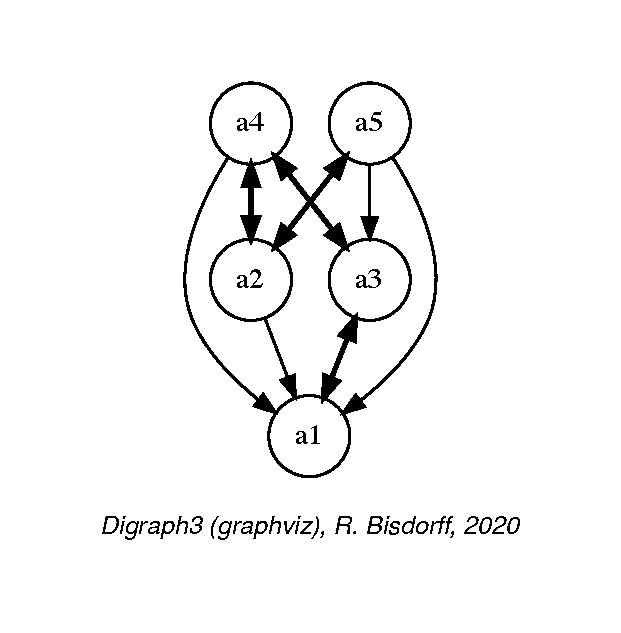
\includegraphics[width=7cm]{Figures/1-1-tutorialDigraph.pdf}
\caption{The tutorial crisp digraph. The \texttt{exportGraphViz()} method is depending on drawing tools from \texttt{https://graphviz.org}. On Linux Ubuntu or Debian you may try '\texttt{sudo apt-get install graphviz}’ to install them. For Mac OSX There are ready $dmg$ installers available}
\label{fig:1.1}       % Give a unique label
\end{figure}

Further methods are provided for inspecting this random \texttt{Digraph} object \texttt{dg}, like the following \texttt{showStatistics()}\index{showStatistics@\texttt{showStatistics()}} method.
\begin{lstlisting}[caption={Inspecting a \texttt{Digraph} object},label=list:1.5]
>>> dg.showStatistics()
 *----- general statistics -------------*
 for digraph              : <tutorialDigraph.py>
 order                    : 5 nodes
 size                     : 12 arcs
 undetermined           : 0 arcs
 determinateness (%)      : 100.0
 arc density              : 0.60
 double arc density       : 0.40
 single arc density       : 0.40
 absence density          : 0.20
 strict single arc density: 0.40
 strict absence density   : 0.20
 nbr. of components         : 1
 nbr. of strong components  : 1
 transitivity degree (%)  : 60.0
                          : [0, 1, 2, 3, 4, 5]
 outdegrees distribution  : [0, 1, 1, 3, 0, 0]
 indegrees distribution   : [0, 1, 2, 1, 1, 0]
 mean outdegree           : 2.40
 mean indegree            : 2.40
                          : [0, 1, 2, 3, 4, 5, 6, 7, 8, 9, 10]
 symmetric degrees dist.  : [0, 0, 0, 0, 1, 4, 0, 0, 0, 0, 0]
 mean symmetric degree    : 4.80
 outdegrees concentration index   : 0.1667
 indegrees concentration index    : 0.2333
 symdegrees concentration index   : 0.0333
                                  : [0, 1, 2, 3, 4, 'inf']
 neighbourhood depths distribution: [0, 1, 4, 0, 0, 0]
 mean neighbourhood depth         : 1.80
 digraph diameter                 : 2
 agglomeration distribution       :
 a1 : 58.33
 a2 : 33.33
 a3 : 33.33
 a4 : 50.00
 a5 : 50.00
 agglomeration coefficient        : 45.00
\end{lstlisting}

The preceding \texttt{show...()} methods usually rely upon corresponding compute methods, like: \texttt{computeSize()}\index{computeSize@\texttt{computeSize()}}, \texttt{computeDeterminateness()}\index{computeDeterminateness@\texttt{computeDeterminateness()}},\\ or \texttt{computeTransitivityDegree()}\index{computeTransitivityDegree@\texttt{computeTransitivityDegree()}}.
\begin{lstlisting}[caption={Various \texttt{compute...()} methods.},label=list:1.6]
>>> dg.computeSize()
 12
>>> dg.computeDeterminateness(InPercents=True)
 Decimal('100.00')
>>> dg.computeTransitivityDegree(InPercents=True)
 Decimal('60.00')
\end{lstlisting}

Mind that \texttt{show...()} methods output their results in the \emph{Python} console. We provide also some \texttt{showHTML...()} methods which output their results in a system browser’s tab or window.
\begin{lstlisting}
>>> dg.showHTMLRelationMap(relationName='r(x,y)',\
...                        rankingRule=None)
\end{lstlisting}
\begin{figure}[ht]
\sidecaption[t]
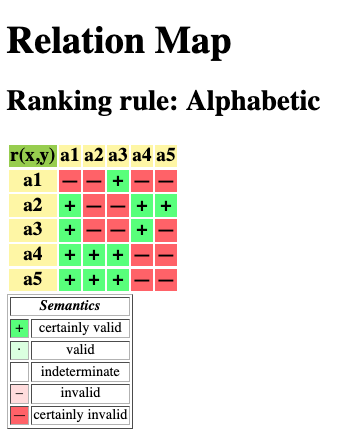
\includegraphics[width=5cm]{Figures/1-2-relationMap1.png}
\caption{Browsing the relation map of the tutorial digraph. $+$ indicates a certainly valid and $-$ indicates a certainly  invalid relation, Here we find confirmed again that our random digraph instance \texttt{dg}, is indeed a crisp, i.e. $100\%$ determined irreflexive digraph instance}
\label{fig:1.2}       % Give a unique label
\end{figure}

% \section{Special digraph instances}
% \label{sec:1.5}

Some special types of digraph instances, like the \texttt{CirculantDigraph}\index{CirculantDigraph@\texttt{CirculantDigraph} class} or the \texttt{GridDigraph}\index{GridDigraph@texttt{GridDigraph} class} classes, are readily available (see Fig.~\vref{fig:1.3}).
 \begin{figure}[ht]
%\sidecaption[t]
  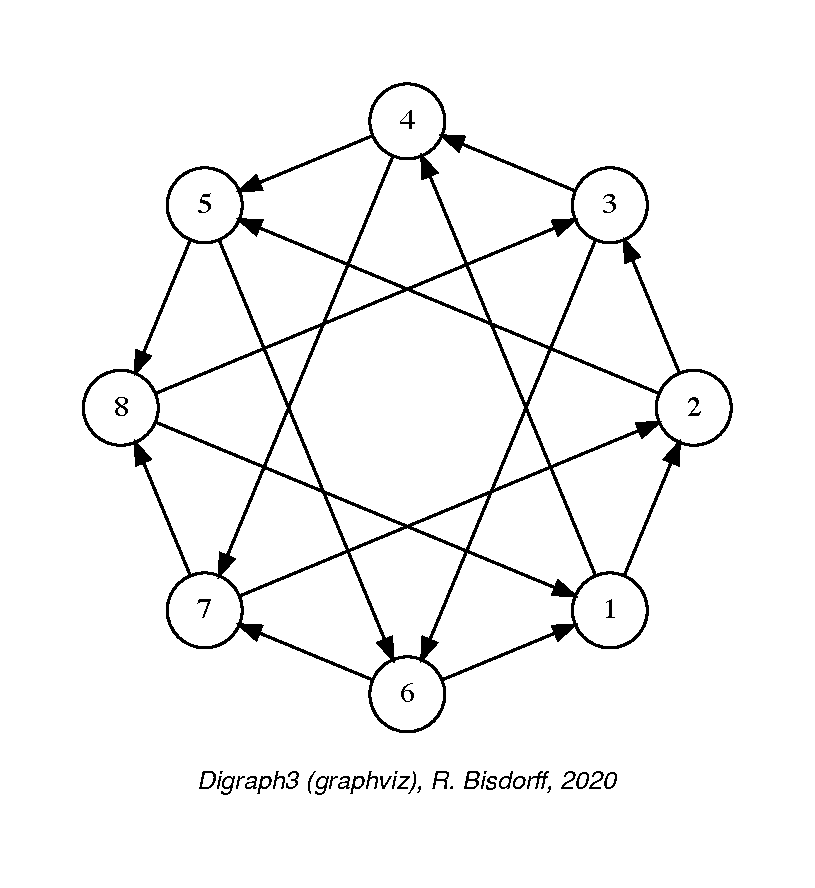
\includegraphics[height=6cm]{Figures/1-3-c8.pdf} \hfill
  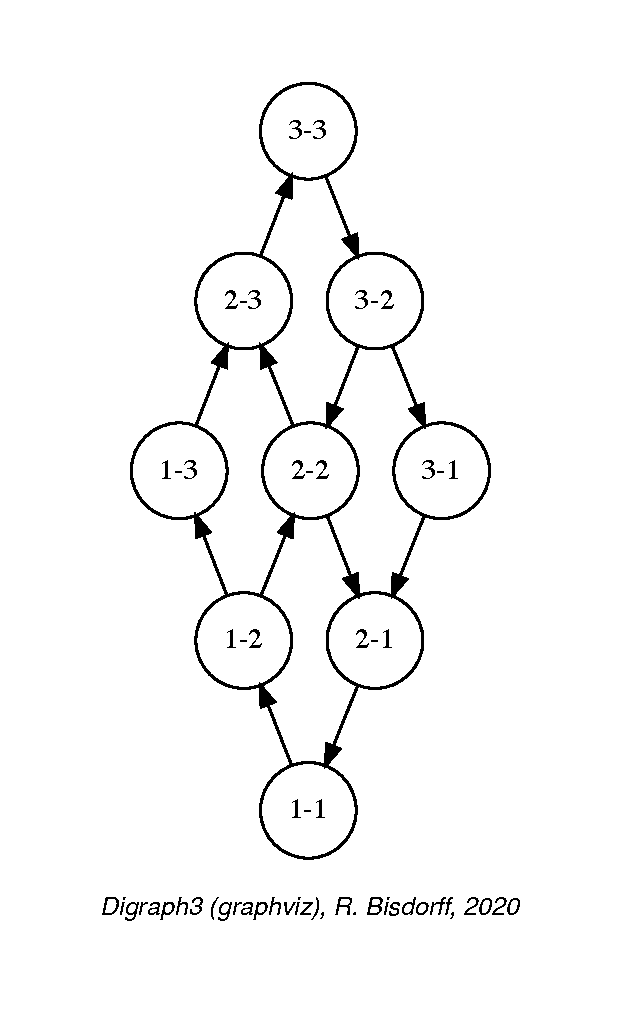
\includegraphics[height=6cm]{Figures/1-3-grid3.pdf} \hfill
  \caption{The circulant [1,3] digraph and the 3x3 grid digraph}
\label{fig:1.3}       % Give a unique label
\end{figure}
\begin{lstlisting}[caption={Circulant digraphs and $n \times m$ grid digraphs},label=list:1.7]
>>> from digraphs import CirculantDigraph,GridDigraph
>>> c8 = CirculantDigraph(order=8,circulants=[1,3])
>>> c8.exportGraphViz('c8')
  *---- exporting a dot file for GraphViz tools ----*
   Exporting to c8.dot
   circo -Tpng c8.dot -o c8.png
>>> grid3 = GridDigraph(n=3,m=3,\
...                    hasMedianSplitOrientation=True)
>>> grid.exportGraphViz('grid3')
  *---- exporting a dot file for GraphViz tools ----*
   Exporting to grid3.dot
   dot -Grankdir=BT -Tpng grid3.dot -o grid3.png
 \end{lstlisting}

\vspace{1cm}
The next Chapter~\ref{sec:2} will introduce the fondamental \emph{bipolar-valued digraph} model which is \emph{root object type} to all the digraph models implemented in the \Digraph modules \citep{BIS-2021b}.    

%%%%%%% The chapter bibliography
% % \normallatexbib
\bibliographystyle{spbasic}
\bibliography{03-backMatters/reference}
%\phantomsection
%\addcontentsline{toc}{section}{Chapter Bibliography}
%%%%%%%%%%%%%%%%%%%%%% chapter.tex %%%%%%%%%%%%%%%%%%%%%%%%%%%%%%%%%
%
% sample chapter
%
% Use this file as a template for your own input.
%
%%%%%%%%%%%%%%%%%%%%%%%% Springer-Verlag %%%%%%%%%%%%%%%%%%%%%%%%%%
%\motto{Use the template \emph{chapter.tex} to style the various elements of your chapter content.}
\chapter{Working with the \Digraph Python resources}
\label{sec:1} % chapter1
% use \chaptermark{}
% to alter or adjust the chapter heading in the running head

\abstract*{ The chapter is devoted to a first contact with the \Digraph Python resources. Following the installation instructions, we list the main Python modules with their purpose and eventually illustrate in a first Python terminal session how to generate, save and inspect a random crisp digraph.}

\abstract{ The chapter is devoted to a first contact with the \Digraph Python resources. Following the installation instructions, we list the main Python modules with their purpose and eventually illustrate in a first Python terminal session how to generate, save and inspect a random crisp digraph.}

\section{Installing the \Digraph resources}
\label{sec:1.1}

Using the \Digraph Python modules is easy\footnote{See the technical description of the \Digraph programming resources, \citet{BIS-2021b}.}. You only need to have installed on your system the Python programming language of version 3 (readily available under Linux and Mac OS). Notice that, from Version 3.3 on, the Python standard \texttt{decimal} module implements very efficiently in C its \texttt{Decimal} class. Now, \texttt{Decimal} numbers are mainly used in the \Digraph characteristic valuation functions, which makes the recent \texttt{Python-3.7+} versions much faster (more than twice as fast) when extensive digraph operations are performed.
%\lstset{style=shstyle}
Several download options (easiest under Linux or Mac OS-X) are given; either, by using a git client and clone a working copy from the \texttt{github.com} directory:
\begin{lstlisting}[language=sh, backgroundcolor=\color{White}, numbers=none]
  ...$ git clone https://github.com/rbisdorff/Digraph3
\end{lstlisting}
or from the \texttt{sourceforge.net} directory:
\begin{lstlisting}[language=sh,backgroundcolor=\color{White},numbers=none]
  ...$ git clone https://git.code.sf.net/p/digraph3/code Digraph3
\end{lstlisting}

It is also possible with a browser access, to download either, from the \texttt{github.com} link or, from the \texttt{sourceforge.net} link above the latest distribution zip archive and extract it.

On Linux or Mac OS, \texttt{..\$ cd} to the cloned or extracted \texttt{Digraph3} directory. The following shell command installs (with \emph{sudo} !) the \Digraph modules in the current running python environment:
\begin{lstlisting}[language=sh, backgroundcolor=\color{White},numbers=none]
  .../Digraph3$ make install
\end{lstlisting}

Python-3.8 (or later) environment is recommended (see the \texttt{makefile} for adapting the \texttt{make install} command to your running python environment).

Whereas the following shell command installs the \Digraph modules in an activated virtual python environment:
\begin{lstlisting}[language=sh, backgroundcolor=\color{White}, numbers=none]
  .../Digraph3$ make installVenv
\end{lstlisting}


If the \emph{cython} \footnote{\href{https://cython.org}{https://cython.org}} C-compiled modules for Big Data applications are required, it is necessary to previously install the \emph{Cython} package in the running Python environment:
\begin{lstlisting}[language=sh, backgroundcolor=\color{White}, numbers=none]
  ...$ python3 -m pip install cython
\end{lstlisting}

It is recommended to run a test suite:
\begin{lstlisting}[language=sh, backgroundcolor=\color{White}, numbers=none]
  .../Digraph3$ make tests
\end{lstlisting}

Test results are stored in the \texttt{Digraph3/test} directory. Notice that the python3 \texttt{pytest} package is required:
\begin{lstlisting}[language=sh, backgroundcolor=\color{White}, numbers=none]
  ...$ python3 -m pip install pytest
\end{lstlisting}

A verbose (with \texttt{stdout} not captured) \texttt{pytest} suite may be run as follows:
\begin{lstlisting}[language=sh, backgroundcolor=\color{White}, numbers=none]
  .../Digraph3$ make verboseTests
\end{lstlisting}

When the GNU \texttt{parallel} shell tool\index{parallel@\texttt{parallel} shell tool}\footnote{\href{https://www.gnu.org/software/parallel}{https://www.gnu.org/software/parallel}} is installed and multiple cores are detected, the tests may be executed in multiple processing mode:
\begin{lstlisting}[language=sh, backgroundcolor=\color{White}, numbers=none]
  ../Digraph3$ make pTests
\end{lstlisting}

Individual module \texttt{pytest} suites are also provided (see the \texttt{makefile}), like the one for the \texttt{outrankingDigraphs} module (see Chap.~\ref{sec:2}):
\begin{lstlisting}[language=sh, backgroundcolor=\color{White}, numbers=none]
../Digraph3$ make outrankingDigraphsTests
\end{lstlisting}

\paragraph{\textbf{Dependencies:}}

\noindent To be fully functional, the \Digraph resources mainly need:
\begin{itemize}[leftmargin=0.5cm,listparindent=0em,rightmargin=0.2cm,topsep=1pt]
\item The \texttt{graphviz} tools \citep{graphviz}\footnote{\href{https://graphviz.org}{https://graphviz.org}}, and 
\item The R statistics resources \footnote{\href{https://www.r-project.org}{https://www.r-project.org}} to be installed.
\item When exploring digraph isomorphisms, the \texttt{nauty} isomorphism testing program is required \citep*{nauty}. On linux you may try: \texttt{sudo apt install nauty}. For Mac OS X, corresponding \texttt{dmg} installers are available for downloading.
\item Two specific methods of the \texttt{OutrankingDigraph} class for clustering performance criteria or decision alternatives require furthermore the \texttt{calmat} matrix computing resource to be installed (see the \texttt{calmat} directory in the \Digraph resources).
\end{itemize}

\section{Organisation of the \Digraph Python modules}
\label{sec:1.2}

The main data handling modules of the \Digraph resources are the following:
\begin{enumerate}[leftmargin=0.75cm]
\item \texttt{digraphs}: main part of the \Digraph source code with the root \texttt{Digraph} class.
\item \texttt{graphs}: resources for handling undirected graphs with the root \texttt{Graph} class and a bridge to the \texttt{digraphs} module resources.
\item \texttt{perfTabs}: tools for handling multiple-criteria performance tableaux with root \texttt{PerformanceTableau} class.
\item \texttt{outrankingDigraphs}: root module for handling outranking digraphs with the abstract root \texttt{OutrankingDigraph} class and the main \texttt{Bipolar\-OutrankingDigraph} class. \footnote{Notice that the outrankingDigraph class defines a hybrid object type, inheriting conjointly from the \texttt{Digraph} class and the \texttt{PerformanceTableau} class.}
\item \texttt{votingProfiles}: classes and methods for handling voting ballots and computing election results with main \texttt{LinearVotingProfile} class.
\end{enumerate}

\noindent Various random generators are provided by the following modules:
\begin{enumerate}[leftmargin=0.75cm]
\item \texttt{randomDigraphs}: various random digraph models like random crisp digraphs (\texttt{RandomDigraph} class) or random bipolar-valued digraphs (\texttt{Random\-ValuationDigraph} class).
\item \texttt{randomPerfTabs}: various implemented random performance tableau models, like Cost-Benefit tableaux (\texttt{RandomCBPerformance\-Tableau} class) or 3-Objectives tableaux (\texttt{Random3ObjectivesPer\-formance\-Tableau} class).
\item \texttt{randomNumbers}: additional random number generators, not available in the standard Python \texttt{random.py} library, like a discrete random variable (\texttt{DiscreteRandomVariable} class) or a Cauchy random variable (\texttt{Cau\-chy\-RandomVariable} class)
\end{enumerate}

\noindent Following modules provide tools for \emph{sorting}, \emph{ranking} and \emph{rating} problems:
\begin{enumerate}[leftmargin=0.75cm]
\item \texttt{sortingDigraphs}: tools for solving sorting problems with the root \texttt{Sor\-tingDigraph} class and the main \texttt{QuantilesSortingDi\-graph} class;
\item \texttt{linearOrders}: tools for solving linearly ranking or ordering problems with the root \texttt{LinearOrder} class;
\item \texttt{transitiveDigraphs}: additional tools for handing transitive digraphs with root \texttt{TransitiveDigraph} class.
\end{enumerate}

\noindent Tools for specifically handling Big Data are eventually provided by the following modules:
\begin{enumerate}[leftmargin=0.75cm]
\item \texttt{performanceQuantiles}: incremental representation of large performance tableaux via binned cumulated density functions per criteria; Depends on the \texttt{randomPerfTabs} module.
\item \texttt{sparseOutrankingDigraphs}: sparse implementation design for bipolar-valued outranking digraphs of order $> 500$.
\item \emph{Cythonized} modules: C-compiled and optimised Python modules for handling big performance tableaux and bipolar outranking digraphs of order $> 1000$.
\end{enumerate}

Readers interested in technical implementation details are invited to consult the reference manual of the \Digraph resources, where they will find the documentation and complete source code of all \Digraph modules, classes and methods \citep{BIS-2021b}. 

\section{Starting a \Digraph terminal session}
\label{sec:1.3}
After downloading the \Digraph resources, one may start an interactive Python3 terminal session in the \texttt{Digraph3} directory.
\begin{lstlisting}[language=sh, backgroundcolor=\color{White}, numbers=none]
  $HOME/.../Digraph3$ python3
  Python 3.9.6 (v3.9.6:db3ff76da1, Jun 28 2021, 11:49:53) 
  [Clang 6.0 (clang-600.0.57)] on darwin
  Type "help", "copyright", "credits" or 
     "license" for more information.
  >>>
\end{lstlisting}

For exploring the classes and methods provided by the \Digraph modules enter the Python3 commands following the session prompts marked with $>>>$ or \texttt{...}; the lines without a prompt are output from the Python3 interpreter. Python class names and boolean parameters start by convention with a capital case; names of other Python objects, like modules, methods and variables start with a lower case. All Python names and code are shown in a \texttt{typewriting} font.
\begin{lstlisting}[caption={Generating a digraph instance},label=list:1.1]
>>> from randomDigraphs import RandomDigraph
>>> dg = RandomDigraph(order=5,arcProbability=0.5,\
...                    seed=101)
>>> dg
  *------- Digraph instance description ------*
   Instance class      : RandomDigraph
   Instance name       : randomDigraph
   Digraph Order       : 5
   Digraph Size        : 12
   Valuation domain    : [-1.00; 1.00]
   Determinateness (%) : 100.00
   Attributes       : ['actions','valuationdomain',
                       'relation','order','name',
                       'gamma','notGamma']
\end{lstlisting}

In Listing~\vref{list:1.1}  we import, for instance, from the \texttt{randomDigraphs}\index{randomDigraphs@\texttt{randomDigraphs} module} module the \texttt{RandomDigraph} class \index{RandomDigraph@\texttt{RandomDigraph} class} in order to generate a random digraph object \texttt{dg} of order 5 and arc probability of $50\%$. The resulting digraph of \emph{order} 5 --number of nodes called (decision) \emph{actions}-- and \emph{size} 12 --number of arcs-- is completely determined (see Line 11) .

% \section{Permanent storage of a digraph object}
% \label{sec:1.3}                   
The content of \texttt{dg} may be saved in a file named \texttt{tutorialDigraph.py}.
\begin{lstlisting}
>>> dg.save('tutorialDigraph')
 *--- Saving digraph in file: <tutorialDigraph.py> ---*
\end{lstlisting}
with the following content:
\begin{lstlisting}[caption={A stored digraph instance},label=list:1.2]
from decimal import Decimal
from collections import OrderedDict
actions = OrderedDict([
    ('a1', {'shortName': 'a1',
          'name': 'random decision action'}),
    ('a2', {'shortName': 'a2',
          'name': 'random decision action'}),
    ('a3', {'shortName': 'a3',
          'name': 'random decision action'}),
    ('a4', {'shortName': 'a4',
          'name': 'random decision action'}),
    ('a5', {'shortName': 'a5',
          'name': 'random decision action'}),
 ])
valuationdomain = {
     'min': Decimal('-1.0'),
     'med': Decimal('0.0'),
     'max': Decimal('1.0'),
     'hasIntegerValuation': True, # representation format
 }
relation = {
     'a1': {'a1':Decimal('-1.0'), 'a2':Decimal('-1.0'),
              'a3':Decimal('1.0'), 'a4':Decimal('-1.0'),
              'a5':Decimal('-1.0'),},
     'a2': {'a1':Decimal('1.0'), 'a2':Decimal('-1.0'),
              'a3':Decimal('-1.0'), 'a4':Decimal('1.0'),
              'a5':Decimal('1.0'),},
     'a3': {'a1':Decimal('1.0'), 'a2':Decimal('-1.0'),
              'a3':Decimal('-1.0'), 'a4':Decimal('1.0'),
              'a5':Decimal('-1.0'),},
     'a4': {'a1':Decimal('1.0'), 'a2':Decimal('1.0'),
              'a3':Decimal('1.0'), 'a4':Decimal('-1.0'),
              'a5':Decimal('-1.0'),},
     'a5': {'a1':Decimal('1.0'), 'a2':Decimal('1.0'),
              'a3':Decimal('1.0'), 'a4':Decimal('-1.0'),
              'a5':Decimal('-1.0'),},
 }
\end{lstlisting}

In the \Digraph resources, all digraph object instances are of root \texttt{Digraph}\index{Digraph@\texttt{Digraph} class} type (\href{https://digraph3.readthedocs.io/en/latest/techDoc.html#organisation-of-the-digraph3-modules}{see the technical description}) and contain at least the following attributes (see Listing~\vref{list:1.1}  Lines 12-14):
\begin{enumerate}[leftmargin=0.5cm,listparindent=0em,nosep]
\item A \texttt{name} attribute, holding usually the actual name of the stored instance that was used to create the instance;
\item An ordered dictionary of digraph nodes called \texttt{actions} (decision alternatives) with at least a \texttt{name} attribute;
\item An \texttt{order} attribute containing the number of graph nodes (length of the actions dictionary) automatically added by the object constructor;
\item  A logical characteristic \texttt{valuationdomain} dictionary with three decimal entries: the minimum ($-1.0$, means certainly false), the median ($0.0$, means missing information) and the maximum characteristic value ($+1.0$, means certainly true);
\item A double dictionary called \texttt{relation} and indexed by an oriented pair of actions (nodes) and carrying a decimal characteristic value in the range of the previous valuation domain;
\item Its associated \texttt{gamma } attribute, a dictionary containing the direct successors, respectively predecessors of each action, automatically added by the object constructor;
\item Its associated \texttt{notGamma} attribute, a dictionary containing the actions that are not direct successors respectively predecessors of each action, automatically added by the object constructor.
\end{enumerate}

\section{Inspecting a digraph object}
\label{sec:1.4}

Different \texttt{show...()} methods, like the \texttt{showShort()} method \index{showShort@\texttt{showShort()}}, reveal us now that \texttt{dg} is a crisp, irreflexive and connected digraph of order five (see List.~\vref{list:1.3}  Lines 1, 16, 26, 29).

\begin{lstlisting}[caption={Random crisp digraph object},label=list:1.3]
>>> dg.showShort()
 *----- show short -------------*
 Digraph          : tutorialDigraph
 Actions          : OrderedDict([
  ('a1', {'shortName': 'a1', 'name': 'random decision action'}),
  ('a2', {'shortName': 'a2', 'name': 'random decision action'}),
  ('a3', {'shortName': 'a3', 'name': 'random decision action'}),
  ('a4', {'shortName': 'a4', 'name': 'random decision action'}),
  ('a5', {'shortName': 'a5', 'name': 'random decision action'})
  ])
 Valuation domain : {
  'min': Decimal('-1.0'),
  'max': Decimal('1.0'),
  'med': Decimal('0.0'), 'hasIntegerValuation': True
  }
>>> dg.showRelationTable()
 * ---- Relation Table -----
   S   |  'a1'  'a2'  'a3'  'a4'  'a5'
 ------|-------------------------------
  'a1' |   -1    -1     1    -1    -1
  'a2' |    1    -1    -1     1     1
  'a3' |    1    -1    -1     1    -1
  'a4' |    1     1     1    -1    -1
  'a5' |    1     1     1    -1    -1
 Valuation domain: [-1;+1]
>>> dg.showComponents()
 *--- Connected Components ---*
 1: ['a1', 'a2', 'a3', 'a4', 'a5']
>>> dg.showNeighborhoods()
 Neighborhoods:
   Gamma     :
 'a1': in => {'a2', 'a4', 'a3', 'a5'}, out => {'a3'}
 'a2': in => {'a5', 'a4'}, out => {'a1', 'a4', 'a5'}
 'a3': in => {'a1', 'a4', 'a5'}, out => {'a1', 'a4'}
 'a4': in => {'a2', 'a3'}, out => {'a1', 'a3', 'a2'}
 'a5': in => {'a2'}, out => {'a1', 'a3', 'a2'}
   Not Gamma :
 'a1': in => set(), out => {'a2', 'a4', 'a5'}
 'a2': in => {'a1', 'a3'}, out => {'a3'}
 'a3': in => {'a2'}, out => {'a2', 'a5'}
 'a4': in => {'a1', 'a5'}, out => {'a5'}
 'a5': in => {'a1', 'a4', 'a3'}, out => {'a4'}
\end{lstlisting}

The \texttt{exportGraphViz()}\index{exportGraphViz@\texttt{exportGraphViz()}} method generates in the current working directory a \texttt{tutorialDigraph.dot} file and a \texttt{tutorialdigraph.png} picture of the tutorial digraph \texttt{dg} (see Fig.~\vref{fig:1.1}), if the \emph{graphviz} tools are installed on your system \citep{graphviz}.
\begin{lstlisting}
>>> dg.exportGraphViz('tutorialDigraph')
 *---- exporting a dot file do GraphViz tools ---------*
 Exporting to tutorialDigraph.dot
 dot -Grankdir=BT -Tpng tutorialDigraph.dot -o tutorialDigraph.png
\end{lstlisting}
\begin{figure}[ht]
\sidecaption[t]
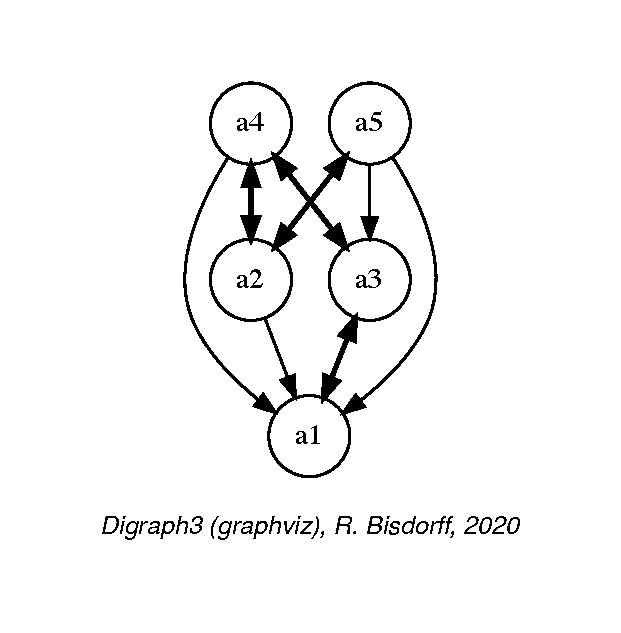
\includegraphics[width=7cm]{Figures/1-1-tutorialDigraph.pdf}
\caption[The tutorial crisp digraph]{The tutorial crisp digraph. The \texttt{exportGraphViz()} method is depending on drawing tools from \texttt{https://graphviz.org}. On Linux Ubuntu or Debian you may try '\texttt{sudo apt-get install graphviz}’ to install them. For Mac OSX There are ready $dmg$ installers available}
\label{fig:1.1}       % Give a unique label
\end{figure}

Further methods are provided for inspecting this random \texttt{Digraph} object \texttt{dg}, like the following \texttt{showStatistics()}\index{showStatistics@\texttt{showStatistics()}} method.
\begin{lstlisting}[caption={Inspecting a \texttt{Digraph} object},label=list:1.5]
>>> dg.showStatistics()
 *----- general statistics -------------*
 for digraph              : <tutorialDigraph.py>
 order                    : 5 nodes
 size                     : 12 arcs
 undetermined           : 0 arcs
 determinateness (%)      : 100.0
 arc density              : 0.60
 double arc density       : 0.40
 single arc density       : 0.40
 absence density          : 0.20
 strict single arc density: 0.40
 strict absence density   : 0.20
 nbr. of components         : 1
 nbr. of strong components  : 1
 transitivity degree (%)  : 60.0
                          : [0, 1, 2, 3, 4, 5]
 outdegrees distribution  : [0, 1, 1, 3, 0, 0]
 indegrees distribution   : [0, 1, 2, 1, 1, 0]
 mean outdegree           : 2.40
 mean indegree            : 2.40
                          : [0, 1, 2, 3, 4, 5, 6, 7, 8, 9, 10]
 symmetric degrees dist.  : [0, 0, 0, 0, 1, 4, 0, 0, 0, 0, 0]
 mean symmetric degree    : 4.80
 outdegrees concentration index   : 0.1667
 indegrees concentration index    : 0.2333
 symdegrees concentration index   : 0.0333
                                  : [0, 1, 2, 3, 4, 'inf']
 neighbourhood depths distribution: [0, 1, 4, 0, 0, 0]
 mean neighbourhood depth         : 1.80
 digraph diameter                 : 2
 agglomeration distribution       :
 a1 : 58.33
 a2 : 33.33
 a3 : 33.33
 a4 : 50.00
 a5 : 50.00
 agglomeration coefficient        : 45.00
\end{lstlisting}

The preceding \texttt{show...()} methods usually rely upon corresponding compute methods, like: \texttt{computeSize()}\index{computeSize@\texttt{computeSize()}}, \texttt{computeDeterminateness()}\index{computeDeterminateness@\texttt{computeDeterminateness()}},\\ or \texttt{computeTransitivityDegree()}\index{computeTransitivityDegree@\texttt{computeTransitivityDegree()}}.
\begin{lstlisting}[caption={Various \texttt{compute...()} methods.},label=list:1.6]
>>> dg.computeSize()
 12
>>> dg.computeDeterminateness(InPercents=True)
 Decimal('100.00')
>>> dg.computeTransitivityDegree(InPercents=True)
 Decimal('60.00')
\end{lstlisting}

Mind that \texttt{show...()} methods output their results in the \emph{Python} console. We provide also some \texttt{showHTML...()} methods which output their results in a system browser’s tab or window.
\begin{lstlisting}
>>> dg.showHTMLRelationMap(relationName='r(x,y)',\
...                        rankingRule=None)
\end{lstlisting}
\begin{figure}[ht]
\sidecaption[t]
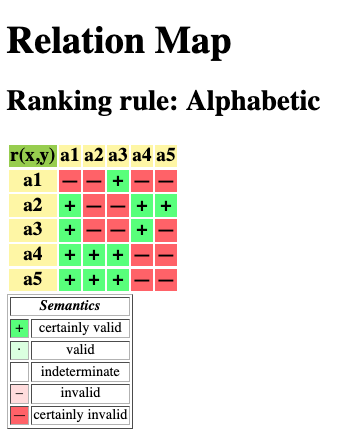
\includegraphics[width=5cm]{Figures/1-2-relationMap1.png}
\caption[Browsing the relation map of the tutorial digraph]{Browsing the relation map of the tutorial digraph. $+$ indicates a certainly valid and $-$ indicates a certainly  invalid relation, Here we find confirmed again that our random digraph instance \texttt{dg}, is indeed a crisp, i.e. $100\%$ determined irreflexive digraph instance}
\label{fig:1.2}       % Give a unique label
\end{figure}

% \section{Special digraph instances}
% \label{sec:1.5}

Some special types of digraph instances, like the \texttt{CirculantDigraph}\index{CirculantDigraph@\texttt{CirculantDigraph} class} or the \texttt{GridDigraph}\index{GridDigraph@\texttt{GridDigraph} class} classes, are readily available (see Fig.~\vref{fig:1.3}).
 \begin{figure}[ht]
%\sidecaption[t]
  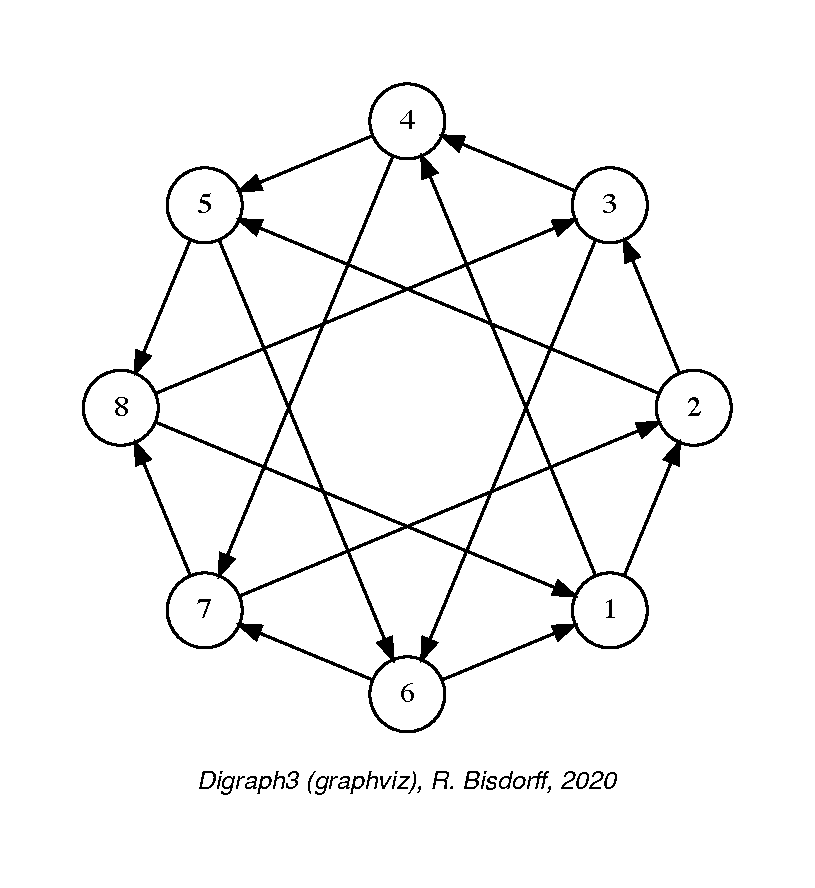
\includegraphics[height=6cm]{Figures/1-3-c8.pdf} \hfill
  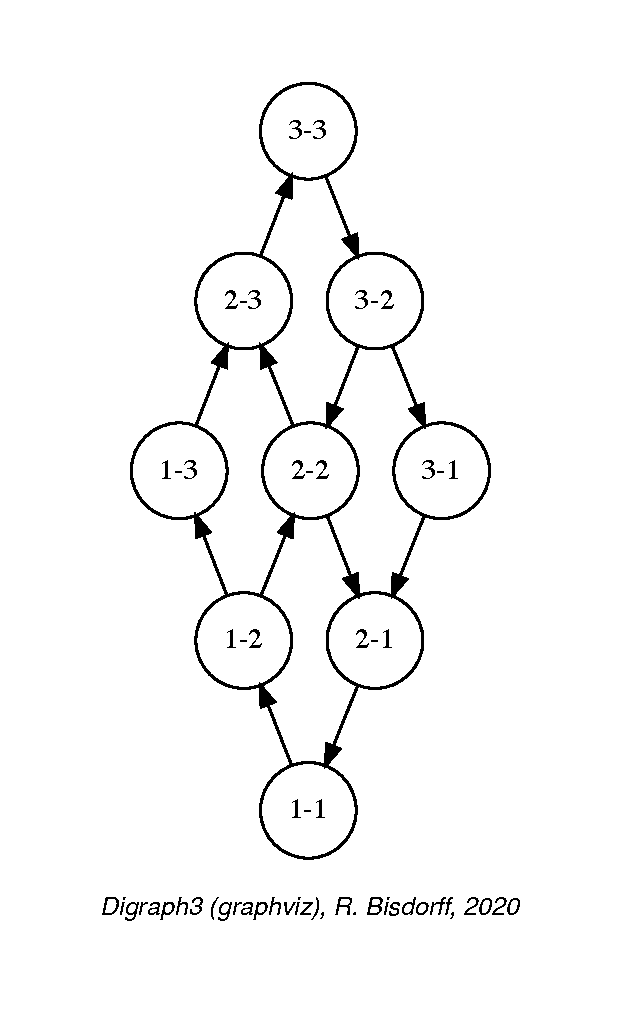
\includegraphics[height=6cm]{Figures/1-3-grid3.pdf} \hfill
  \caption{The circulant [1,3] digraph and the 3x3 grid digraph}
\label{fig:1.3}       % Give a unique label
\end{figure}
\begin{lstlisting}[caption={Circulant digraphs and $n \times m$ grid digraphs},label=list:1.7]
>>> from digraphs import CirculantDigraph,GridDigraph
>>> c8 = CirculantDigraph(order=8,circulants=[1,3])
>>> c8.exportGraphViz('c8')
  *---- exporting a dot file for GraphViz tools ----*
   Exporting to c8.dot
   circo -Tpng c8.dot -o c8.png
>>> grid3 = GridDigraph(n=3,m=3,\
...                    hasMedianSplitOrientation=True)
>>> grid.exportGraphViz('grid3')
  *---- exporting a dot file for GraphViz tools ----*
   Exporting to grid3.dot
   dot -Grankdir=BT -Tpng grid3.dot -o grid3.png
 \end{lstlisting}

%\vspace{1cm}
\vspace{\baselineskip}
The next Chapter~\ref{sec:2} will introduce the fondamental \emph{bipolar-valued digraph} model which is \emph{root object type} to all the digraph models implemented in the \Digraph modules \citep{BIS-2021b}.    

%%%%%%% The chapter bibliography
% % \normallatexbib
%\phantomsection
%\addcontentsline{toc}{section}{Chapter Bibliography}
%%%%%%%%%%%%%%%%%%%%%% chapter.tex %%%%%%%%%%%%%%%%%%%%%%%%%%%%%%%%%
%
% sample chapter
%
% Use this file as a template for your own input.
%
%%%%%%%%%%%%%%%%%%%%%%%% Springer-Verlag %%%%%%%%%%%%%%%%%%%%%%%%%%
%\motto{Use the template \emph{chapter.tex} to style the various elements of your chapter content.}
\chapter{Working with the \Digraph Python resources}
\label{sec:1} % chapter1
% use \chaptermark{}
% to alter or adjust the chapter heading in the running head

\abstract*{ The chapter is devoted to a first contact with the \Digraph Python resources. Following the installation instructions, we list the main Python modules with their purpose and eventually illustrate in a first Python terminal session how to generate, save and inspect a random crisp digraph.}

\abstract{ The chapter is devoted to a first contact with the \Digraph Python resources. Following the installation instructions, we list the main Python modules with their purpose and eventually illustrate in a first Python terminal session how to generate, save and inspect a random crisp digraph.}

\section{Installing the \Digraph resources}
\label{sec:1.1}

Using the \Digraph Python modules is easy\footnote{See the technical description of the \Digraph programming resources, \citet{BIS-2021b}.}. You only need to have installed on your system the Python programming language of version 3 (readily available under Linux and Mac OS). Notice that, from Version 3.3 on, the Python standard \texttt{decimal} module implements very efficiently in C its \texttt{Decimal} class. Now, \texttt{Decimal} numbers are mainly used in the \Digraph characteristic valuation functions, which makes the recent \texttt{Python-3.7+} versions much faster (more than twice as fast) when extensive digraph operations are performed.
%\lstset{style=shstyle}
Several download options (easiest under Linux or Mac OS-X) are given; either, by using a git client and clone a working copy from the \texttt{github.com} directory:
\begin{lstlisting}[language=sh, backgroundcolor=\color{White}, numbers=none]
  ...$ git clone https://github.com/rbisdorff/Digraph3
\end{lstlisting}
or from the \texttt{sourceforge.net} directory:
\begin{lstlisting}[language=sh,backgroundcolor=\color{White},numbers=none]
  ...$ git clone https://git.code.sf.net/p/digraph3/code Digraph3
\end{lstlisting}

It is also possible with a browser access, to download either, from the \texttt{github.com} link or, from the \texttt{sourceforge.net} link above the latest distribution zip archive and extract it.

On Linux or Mac OS, \texttt{..\$ cd} to the cloned or extracted \texttt{Digraph3} directory. The following shell command installs (with \emph{sudo} !) the \Digraph modules in the current running python environment:
\begin{lstlisting}[language=sh, backgroundcolor=\color{White},numbers=none]
  .../Digraph3$ make install
\end{lstlisting}

Python-3.8 (or later) environment is recommended (see the \texttt{makefile} for adapting the \texttt{make install} command to your running python environment).

Whereas the following shell command installs the \Digraph modules in an activated virtual python environment:
\begin{lstlisting}[language=sh, backgroundcolor=\color{White}, numbers=none]
  .../Digraph3$ make installVenv
\end{lstlisting}


If the \emph{cython} \footnote{\href{https://cython.org}{https://cython.org}} C-compiled modules for Big Data applications are required, it is necessary to previously install the \emph{Cython} package in the running Python environment:
\begin{lstlisting}[language=sh, backgroundcolor=\color{White}, numbers=none]
  ...$ python3 -m pip install cython
\end{lstlisting}

It is recommended to run a test suite:
\begin{lstlisting}[language=sh, backgroundcolor=\color{White}, numbers=none]
  .../Digraph3$ make tests
\end{lstlisting}

Test results are stored in the \texttt{Digraph3/test} directory. Notice that the python3 \texttt{pytest} package is required:
\begin{lstlisting}[language=sh, backgroundcolor=\color{White}, numbers=none]
  ...$ python3 -m pip install pytest
\end{lstlisting}

A verbose (with \texttt{stdout} not captured) \texttt{pytest} suite may be run as follows:
\begin{lstlisting}[language=sh, backgroundcolor=\color{White}, numbers=none]
  .../Digraph3$ make verboseTests
\end{lstlisting}

When the GNU \texttt{parallel} shell tool\index{parallel@\texttt{parallel} shell tool}\footnote{\href{https://www.gnu.org/software/parallel}{https://www.gnu.org/software/parallel}} is installed and multiple cores are detected, the tests may be executed in multiple processing mode:
\begin{lstlisting}[language=sh, backgroundcolor=\color{White}, numbers=none]
  ../Digraph3$ make pTests
\end{lstlisting}

Individual module \texttt{pytest} suites are also provided (see the \texttt{makefile}), like the one for the \texttt{outrankingDigraphs} module (see Chap.~\ref{sec:2}):
\begin{lstlisting}[language=sh, backgroundcolor=\color{White}, numbers=none]
../Digraph3$ make outrankingDigraphsTests
\end{lstlisting}

\paragraph{\textbf{Dependencies:}}

\noindent To be fully functional, the \Digraph resources mainly need:
\begin{itemize}[leftmargin=0.5cm,listparindent=0em,rightmargin=0.2cm,topsep=1pt]
\item The \texttt{graphviz} tools \citep{graphviz}\footnote{\href{https://graphviz.org}{https://graphviz.org}}, and 
\item The R statistics resources \footnote{\href{https://www.r-project.org}{https://www.r-project.org}} to be installed.
\item When exploring digraph isomorphisms, the \texttt{nauty} isomorphism testing program is required \citep*{nauty}. On linux you may try: \texttt{sudo apt install nauty}. For Mac OS X, corresponding \texttt{dmg} installers are available for downloading.
\item Two specific methods of the \texttt{OutrankingDigraph} class for clustering performance criteria or decision alternatives require furthermore the \texttt{calmat} matrix computing resource to be installed (see the \texttt{calmat} directory in the \Digraph resources).
\end{itemize}

\section{Organisation of the \Digraph Python modules}
\label{sec:1.2}

The main data handling modules of the \Digraph resources are the following:
\begin{enumerate}[leftmargin=0.75cm]
\item \texttt{digraphs}: main part of the \Digraph source code with the root \texttt{Digraph} class.
\item \texttt{graphs}: resources for handling undirected graphs with the root \texttt{Graph} class and a bridge to the \texttt{digraphs} module resources.
\item \texttt{perfTabs}: tools for handling multiple-criteria performance tableaux with root \texttt{PerformanceTableau} class.
\item \texttt{outrankingDigraphs}: root module for handling outranking digraphs with the abstract root \texttt{OutrankingDigraph} class and the main \texttt{Bipolar\-OutrankingDigraph} class. \footnote{Notice that the outrankingDigraph class defines a hybrid object type, inheriting conjointly from the \texttt{Digraph} class and the \texttt{PerformanceTableau} class.}
\item \texttt{votingProfiles}: classes and methods for handling voting ballots and computing election results with main \texttt{LinearVotingProfile} class.
\end{enumerate}

\noindent Various random generators are provided by the following modules:
\begin{enumerate}[leftmargin=0.75cm]
\item \texttt{randomDigraphs}: various random digraph models like random crisp digraphs (\texttt{RandomDigraph} class) or random bipolar-valued digraphs (\texttt{Random\-ValuationDigraph} class).
\item \texttt{randomPerfTabs}: various implemented random performance tableau models, like Cost-Benefit tableaux (\texttt{RandomCBPerformance\-Tableau} class) or 3-Objectives tableaux (\texttt{Random3ObjectivesPer\-formance\-Tableau} class).
\item \texttt{randomNumbers}: additional random number generators, not available in the standard Python \texttt{random.py} library, like a discrete random variable (\texttt{DiscreteRandomVariable} class) or a Cauchy random variable (\texttt{Cau\-chy\-RandomVariable} class)
\end{enumerate}

\noindent Following modules provide tools for \emph{sorting}, \emph{ranking} and \emph{rating} problems:
\begin{enumerate}[leftmargin=0.75cm]
\item \texttt{sortingDigraphs}: tools for solving sorting problems with the root \texttt{Sor\-tingDigraph} class and the main \texttt{QuantilesSortingDi\-graph} class;
\item \texttt{linearOrders}: tools for solving linearly ranking or ordering problems with the root \texttt{LinearOrder} class;
\item \texttt{transitiveDigraphs}: additional tools for handing transitive digraphs with root \texttt{TransitiveDigraph} class.
\end{enumerate}

\noindent Tools for specifically handling Big Data are eventually provided by the following modules:
\begin{enumerate}[leftmargin=0.75cm]
\item \texttt{performanceQuantiles}: incremental representation of large performance tableaux via binned cumulated density functions per criteria; Depends on the \texttt{randomPerfTabs} module.
\item \texttt{sparseOutrankingDigraphs}: sparse implementation design for bipolar-valued outranking digraphs of order $> 500$.
\item \emph{Cythonized} modules: C-compiled and optimised Python modules for handling big performance tableaux and bipolar outranking digraphs of order $> 1000$.
\end{enumerate}

Readers interested in technical implementation details are invited to consult the reference manual of the \Digraph resources, where they will find the documentation and complete source code of all \Digraph modules, classes and methods \citep{BIS-2021b}. 

\section{Starting a \Digraph terminal session}
\label{sec:1.3}
After downloading the \Digraph resources, one may start an interactive Python3 terminal session in the \texttt{Digraph3} directory.
\begin{lstlisting}[language=sh, backgroundcolor=\color{White}, numbers=none]
  $HOME/.../Digraph3$ python3
  Python 3.9.6 (v3.9.6:db3ff76da1, Jun 28 2021, 11:49:53) 
  [Clang 6.0 (clang-600.0.57)] on darwin
  Type "help", "copyright", "credits" or 
     "license" for more information.
  >>>
\end{lstlisting}

For exploring the classes and methods provided by the \Digraph modules enter the Python3 commands following the session prompts marked with $>>>$ or \texttt{...}; the lines without a prompt are output from the Python3 interpreter. Python class names and boolean parameters start by convention with a capital case; names of other Python objects, like modules, methods and variables start with a lower case. All Python names and code are shown in a \texttt{typewriting} font.
\begin{lstlisting}[caption={Generating a digraph instance},label=list:1.1]
>>> from randomDigraphs import RandomDigraph
>>> dg = RandomDigraph(order=5,arcProbability=0.5,\
...                    seed=101)
>>> dg
  *------- Digraph instance description ------*
   Instance class      : RandomDigraph
   Instance name       : randomDigraph
   Digraph Order       : 5
   Digraph Size        : 12
   Valuation domain    : [-1.00; 1.00]
   Determinateness (%) : 100.00
   Attributes       : ['actions','valuationdomain',
                       'relation','order','name',
                       'gamma','notGamma']
\end{lstlisting}

In Listing~\vref{list:1.1}  we import, for instance, from the \texttt{randomDigraphs}\index{randomDigraphs@\texttt{randomDigraphs} module} module the \texttt{RandomDigraph} class \index{RandomDigraph@\texttt{RandomDigraph} class} in order to generate a random digraph object \texttt{dg} of order 5 and arc probability of $50\%$. The resulting digraph of \emph{order} 5 --number of nodes called (decision) \emph{actions}-- and \emph{size} 12 --number of arcs-- is completely determined (see Line 11) .

% \section{Permanent storage of a digraph object}
% \label{sec:1.3}                   
The content of \texttt{dg} may be saved in a file named \texttt{tutorialDigraph.py}.
\begin{lstlisting}
>>> dg.save('tutorialDigraph')
 *--- Saving digraph in file: <tutorialDigraph.py> ---*
\end{lstlisting}
with the following content:
\begin{lstlisting}[caption={A stored digraph instance},label=list:1.2]
from decimal import Decimal
from collections import OrderedDict
actions = OrderedDict([
    ('a1', {'shortName': 'a1',
          'name': 'random decision action'}),
    ('a2', {'shortName': 'a2',
          'name': 'random decision action'}),
    ('a3', {'shortName': 'a3',
          'name': 'random decision action'}),
    ('a4', {'shortName': 'a4',
          'name': 'random decision action'}),
    ('a5', {'shortName': 'a5',
          'name': 'random decision action'}),
 ])
valuationdomain = {
     'min': Decimal('-1.0'),
     'med': Decimal('0.0'),
     'max': Decimal('1.0'),
     'hasIntegerValuation': True, # representation format
 }
relation = {
     'a1': {'a1':Decimal('-1.0'), 'a2':Decimal('-1.0'),
              'a3':Decimal('1.0'), 'a4':Decimal('-1.0'),
              'a5':Decimal('-1.0'),},
     'a2': {'a1':Decimal('1.0'), 'a2':Decimal('-1.0'),
              'a3':Decimal('-1.0'), 'a4':Decimal('1.0'),
              'a5':Decimal('1.0'),},
     'a3': {'a1':Decimal('1.0'), 'a2':Decimal('-1.0'),
              'a3':Decimal('-1.0'), 'a4':Decimal('1.0'),
              'a5':Decimal('-1.0'),},
     'a4': {'a1':Decimal('1.0'), 'a2':Decimal('1.0'),
              'a3':Decimal('1.0'), 'a4':Decimal('-1.0'),
              'a5':Decimal('-1.0'),},
     'a5': {'a1':Decimal('1.0'), 'a2':Decimal('1.0'),
              'a3':Decimal('1.0'), 'a4':Decimal('-1.0'),
              'a5':Decimal('-1.0'),},
 }
\end{lstlisting}

In the \Digraph resources, all digraph object instances are of root \texttt{Digraph}\index{Digraph@\texttt{Digraph} class} type (\href{https://digraph3.readthedocs.io/en/latest/techDoc.html#organisation-of-the-digraph3-modules}{see the technical description}) and contain at least the following attributes (see Listing~\vref{list:1.1}  Lines 12-14):
\begin{enumerate}[leftmargin=0.5cm,listparindent=0em,nosep]
\item A \texttt{name} attribute, holding usually the actual name of the stored instance that was used to create the instance;
\item An ordered dictionary of digraph nodes called \texttt{actions} (decision alternatives) with at least a \texttt{name} attribute;
\item An \texttt{order} attribute containing the number of graph nodes (length of the actions dictionary) automatically added by the object constructor;
\item  A logical characteristic \texttt{valuationdomain} dictionary with three decimal entries: the minimum ($-1.0$, means certainly false), the median ($0.0$, means missing information) and the maximum characteristic value ($+1.0$, means certainly true);
\item A double dictionary called \texttt{relation} and indexed by an oriented pair of actions (nodes) and carrying a decimal characteristic value in the range of the previous valuation domain;
\item Its associated \texttt{gamma } attribute, a dictionary containing the direct successors, respectively predecessors of each action, automatically added by the object constructor;
\item Its associated \texttt{notGamma} attribute, a dictionary containing the actions that are not direct successors respectively predecessors of each action, automatically added by the object constructor.
\end{enumerate}

\section{Inspecting a digraph object}
\label{sec:1.4}

Different \texttt{show...()} methods, like the \texttt{showShort()} method \index{showShort@\texttt{showShort()}}, reveal us now that \texttt{dg} is a crisp, irreflexive and connected digraph of order five (see List.~\vref{list:1.3}  Lines 1, 16, 26, 29).

\begin{lstlisting}[caption={Random crisp digraph object},label=list:1.3]
>>> dg.showShort()
 *----- show short -------------*
 Digraph          : tutorialDigraph
 Actions          : OrderedDict([
  ('a1', {'shortName': 'a1', 'name': 'random decision action'}),
  ('a2', {'shortName': 'a2', 'name': 'random decision action'}),
  ('a3', {'shortName': 'a3', 'name': 'random decision action'}),
  ('a4', {'shortName': 'a4', 'name': 'random decision action'}),
  ('a5', {'shortName': 'a5', 'name': 'random decision action'})
  ])
 Valuation domain : {
  'min': Decimal('-1.0'),
  'max': Decimal('1.0'),
  'med': Decimal('0.0'), 'hasIntegerValuation': True
  }
>>> dg.showRelationTable()
 * ---- Relation Table -----
   S   |  'a1'  'a2'  'a3'  'a4'  'a5'
 ------|-------------------------------
  'a1' |   -1    -1     1    -1    -1
  'a2' |    1    -1    -1     1     1
  'a3' |    1    -1    -1     1    -1
  'a4' |    1     1     1    -1    -1
  'a5' |    1     1     1    -1    -1
 Valuation domain: [-1;+1]
>>> dg.showComponents()
 *--- Connected Components ---*
 1: ['a1', 'a2', 'a3', 'a4', 'a5']
>>> dg.showNeighborhoods()
 Neighborhoods:
   Gamma     :
 'a1': in => {'a2', 'a4', 'a3', 'a5'}, out => {'a3'}
 'a2': in => {'a5', 'a4'}, out => {'a1', 'a4', 'a5'}
 'a3': in => {'a1', 'a4', 'a5'}, out => {'a1', 'a4'}
 'a4': in => {'a2', 'a3'}, out => {'a1', 'a3', 'a2'}
 'a5': in => {'a2'}, out => {'a1', 'a3', 'a2'}
   Not Gamma :
 'a1': in => set(), out => {'a2', 'a4', 'a5'}
 'a2': in => {'a1', 'a3'}, out => {'a3'}
 'a3': in => {'a2'}, out => {'a2', 'a5'}
 'a4': in => {'a1', 'a5'}, out => {'a5'}
 'a5': in => {'a1', 'a4', 'a3'}, out => {'a4'}
\end{lstlisting}

The \texttt{exportGraphViz()}\index{exportGraphViz@\texttt{exportGraphViz()}} method generates in the current working directory a \texttt{tutorialDigraph.dot} file and a \texttt{tutorialdigraph.png} picture of the tutorial digraph \texttt{dg} (see Fig.~\vref{fig:1.1}), if the \emph{graphviz} tools are installed on your system \citep{graphviz}.
\begin{lstlisting}
>>> dg.exportGraphViz('tutorialDigraph')
 *---- exporting a dot file do GraphViz tools ---------*
 Exporting to tutorialDigraph.dot
 dot -Grankdir=BT -Tpng tutorialDigraph.dot -o tutorialDigraph.png
\end{lstlisting}
\begin{figure}[ht]
\sidecaption[t]
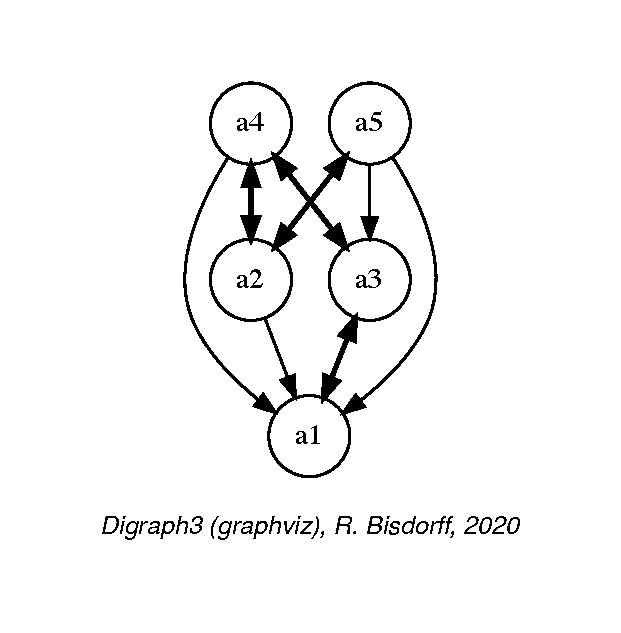
\includegraphics[width=7cm]{Figures/1-1-tutorialDigraph.pdf}
\caption[The tutorial crisp digraph]{The tutorial crisp digraph. The \texttt{exportGraphViz()} method is depending on drawing tools from \texttt{https://graphviz.org}. On Linux Ubuntu or Debian you may try '\texttt{sudo apt-get install graphviz}’ to install them. For Mac OSX There are ready $dmg$ installers available}
\label{fig:1.1}       % Give a unique label
\end{figure}

Further methods are provided for inspecting this random \texttt{Digraph} object \texttt{dg}, like the following \texttt{showStatistics()}\index{showStatistics@\texttt{showStatistics()}} method.
\begin{lstlisting}[caption={Inspecting a \texttt{Digraph} object},label=list:1.5]
>>> dg.showStatistics()
 *----- general statistics -------------*
 for digraph              : <tutorialDigraph.py>
 order                    : 5 nodes
 size                     : 12 arcs
 undetermined           : 0 arcs
 determinateness (%)      : 100.0
 arc density              : 0.60
 double arc density       : 0.40
 single arc density       : 0.40
 absence density          : 0.20
 strict single arc density: 0.40
 strict absence density   : 0.20
 nbr. of components         : 1
 nbr. of strong components  : 1
 transitivity degree (%)  : 60.0
                          : [0, 1, 2, 3, 4, 5]
 outdegrees distribution  : [0, 1, 1, 3, 0, 0]
 indegrees distribution   : [0, 1, 2, 1, 1, 0]
 mean outdegree           : 2.40
 mean indegree            : 2.40
                          : [0, 1, 2, 3, 4, 5, 6, 7, 8, 9, 10]
 symmetric degrees dist.  : [0, 0, 0, 0, 1, 4, 0, 0, 0, 0, 0]
 mean symmetric degree    : 4.80
 outdegrees concentration index   : 0.1667
 indegrees concentration index    : 0.2333
 symdegrees concentration index   : 0.0333
                                  : [0, 1, 2, 3, 4, 'inf']
 neighbourhood depths distribution: [0, 1, 4, 0, 0, 0]
 mean neighbourhood depth         : 1.80
 digraph diameter                 : 2
 agglomeration distribution       :
 a1 : 58.33
 a2 : 33.33
 a3 : 33.33
 a4 : 50.00
 a5 : 50.00
 agglomeration coefficient        : 45.00
\end{lstlisting}

The preceding \texttt{show...()} methods usually rely upon corresponding compute methods, like: \texttt{computeSize()}\index{computeSize@\texttt{computeSize()}}, \texttt{computeDeterminateness()}\index{computeDeterminateness@\texttt{computeDeterminateness()}},\\ or \texttt{computeTransitivityDegree()}\index{computeTransitivityDegree@\texttt{computeTransitivityDegree()}}.
\begin{lstlisting}[caption={Various \texttt{compute...()} methods.},label=list:1.6]
>>> dg.computeSize()
 12
>>> dg.computeDeterminateness(InPercents=True)
 Decimal('100.00')
>>> dg.computeTransitivityDegree(InPercents=True)
 Decimal('60.00')
\end{lstlisting}

Mind that \texttt{show...()} methods output their results in the \emph{Python} console. We provide also some \texttt{showHTML...()} methods which output their results in a system browser’s tab or window.
\begin{lstlisting}
>>> dg.showHTMLRelationMap(relationName='r(x,y)',\
...                        rankingRule=None)
\end{lstlisting}
\begin{figure}[ht]
\sidecaption[t]
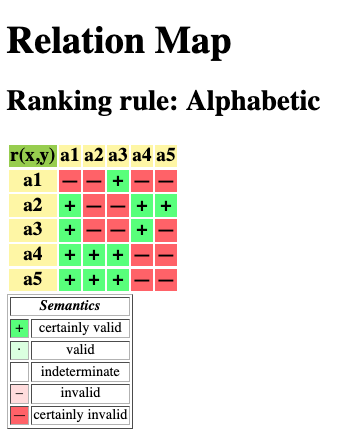
\includegraphics[width=5cm]{Figures/1-2-relationMap1.png}
\caption[Browsing the relation map of the tutorial digraph]{Browsing the relation map of the tutorial digraph. $+$ indicates a certainly valid and $-$ indicates a certainly  invalid relation, Here we find confirmed again that our random digraph instance \texttt{dg}, is indeed a crisp, i.e. $100\%$ determined irreflexive digraph instance}
\label{fig:1.2}       % Give a unique label
\end{figure}

% \section{Special digraph instances}
% \label{sec:1.5}

Some special types of digraph instances, like the \texttt{CirculantDigraph}\index{CirculantDigraph@\texttt{CirculantDigraph} class} or the \texttt{GridDigraph}\index{GridDigraph@\texttt{GridDigraph} class} classes, are readily available (see Fig.~\vref{fig:1.3}).
 \begin{figure}[ht]
%\sidecaption[t]
  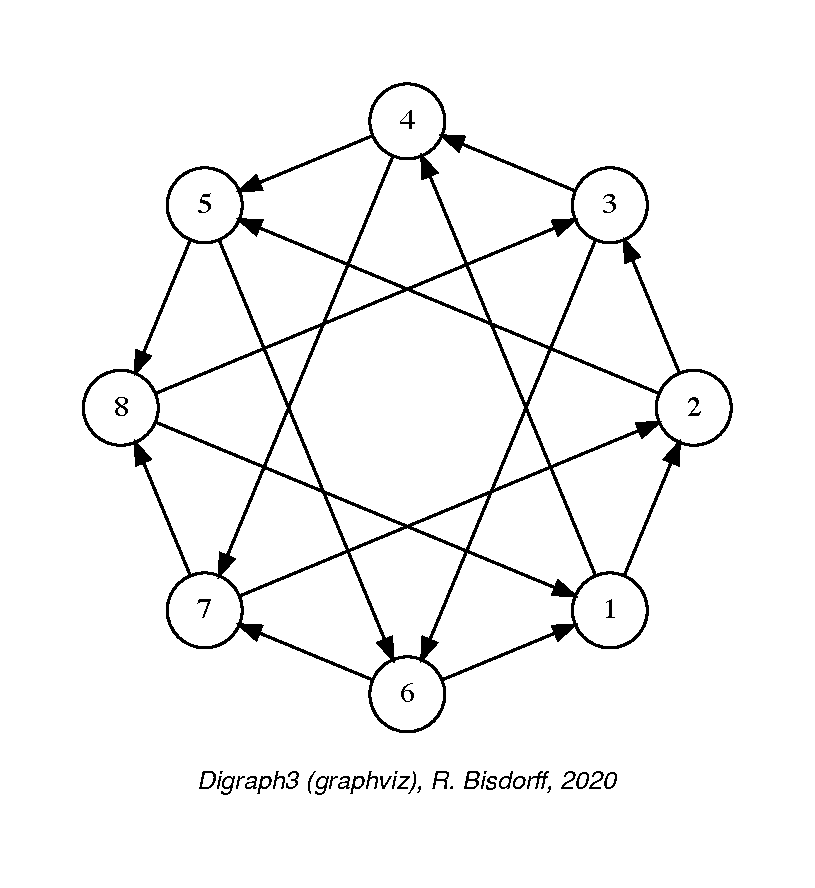
\includegraphics[height=6cm]{Figures/1-3-c8.pdf} \hfill
  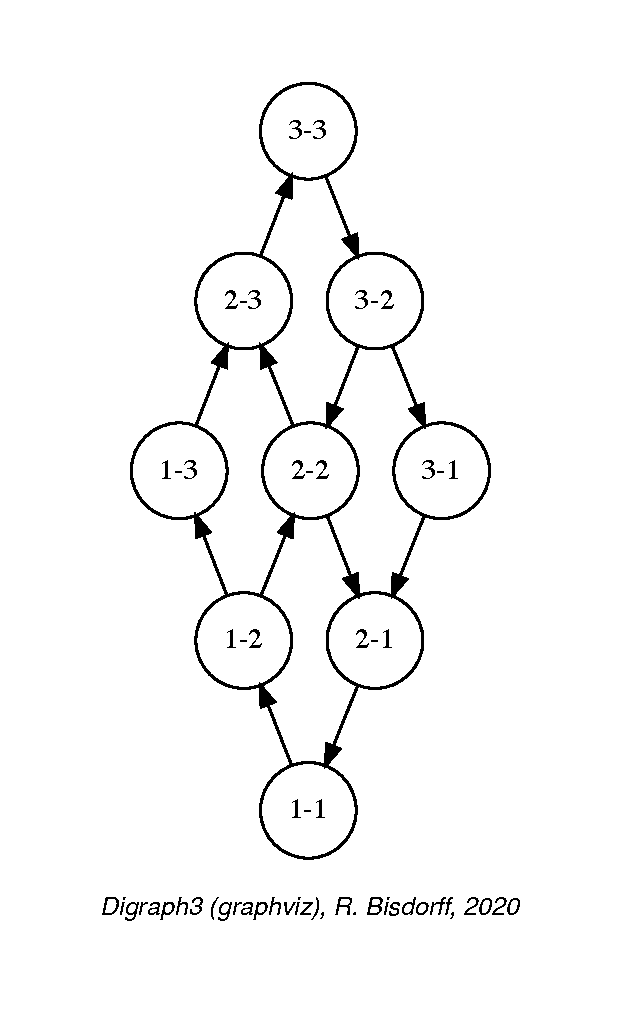
\includegraphics[height=6cm]{Figures/1-3-grid3.pdf} \hfill
  \caption{The circulant [1,3] digraph and the 3x3 grid digraph}
\label{fig:1.3}       % Give a unique label
\end{figure}
\begin{lstlisting}[caption={Circulant digraphs and $n \times m$ grid digraphs},label=list:1.7]
>>> from digraphs import CirculantDigraph,GridDigraph
>>> c8 = CirculantDigraph(order=8,circulants=[1,3])
>>> c8.exportGraphViz('c8')
  *---- exporting a dot file for GraphViz tools ----*
   Exporting to c8.dot
   circo -Tpng c8.dot -o c8.png
>>> grid3 = GridDigraph(n=3,m=3,\
...                    hasMedianSplitOrientation=True)
>>> grid.exportGraphViz('grid3')
  *---- exporting a dot file for GraphViz tools ----*
   Exporting to grid3.dot
   dot -Grankdir=BT -Tpng grid3.dot -o grid3.png
 \end{lstlisting}

%\vspace{1cm}
\vspace{\baselineskip}
The next Chapter~\ref{sec:2} will introduce the fondamental \emph{bipolar-valued digraph} model which is \emph{root object type} to all the digraph models implemented in the \Digraph modules \citep{BIS-2021b}.    

%%%%%%% The chapter bibliography
% % \normallatexbib
%\phantomsection
%\addcontentsline{toc}{section}{Chapter Bibliography}
%%%%%%%%%%%%%%%%%%%%%% chapter.tex %%%%%%%%%%%%%%%%%%%%%%%%%%%%%%%%%
%
% sample chapter
%
% Use this file as a template for your own input.
%
%%%%%%%%%%%%%%%%%%%%%%%% Springer-Verlag %%%%%%%%%%%%%%%%%%%%%%%%%%
%\motto{Use the template \emph{chapter.tex} to style the various elements of your chapter content.}
\chapter{Working with the \Digraph Python resources}
\label{sec:1} % chapter1
% use \chaptermark{}
% to alter or adjust the chapter heading in the running head

\abstract*{ The chapter is devoted to a first contact with the \Digraph Python resources. Following the installation instructions, we list the main Python modules with their purpose and eventually illustrate in a first Python terminal session how to generate, save and inspect a random crisp digraph.}

\abstract{ The chapter is devoted to a first contact with the \Digraph Python resources. Following the installation instructions, we list the main Python modules with their purpose and eventually illustrate in a first Python terminal session how to generate, save and inspect a random crisp digraph.}

\section{Installing the \Digraph resources}
\label{sec:1.1}

Using the \Digraph Python modules is easy\footnote{See the technical description of the \Digraph programming resources, \citet{BIS-2021b}.}. You only need to have installed on your system the Python programming language of version 3 (readily available under Linux and Mac OS). Notice that, from Version 3.3 on, the Python standard \texttt{decimal} module implements very efficiently in C its \texttt{Decimal} class. Now, \texttt{Decimal} numbers are mainly used in the \Digraph characteristic valuation functions, which makes the recent \texttt{Python-3.7+} versions much faster (more than twice as fast) when extensive digraph operations are performed.
%\lstset{style=shstyle}
Several download options (easiest under Linux or Mac OS-X) are given; either, by using a git client and clone a working copy from the \texttt{github.com} directory:
\begin{lstlisting}[language=sh, backgroundcolor=\color{White}, numbers=none]
  ...$ git clone https://github.com/rbisdorff/Digraph3
\end{lstlisting}
or from the \texttt{sourceforge.net} directory:
\begin{lstlisting}[language=sh,backgroundcolor=\color{White},numbers=none]
  ...$ git clone https://git.code.sf.net/p/digraph3/code Digraph3
\end{lstlisting}

It is also possible with a browser access, to download either, from the \texttt{github.com} link or, from the \texttt{sourceforge.net} link above the latest distribution zip archive and extract it.

On Linux or Mac OS, \texttt{..\$ cd} to the cloned or extracted \texttt{Digraph3} directory. The following shell command installs (with \emph{sudo} !) the \Digraph modules in the current running python environment:
\begin{lstlisting}[language=sh, backgroundcolor=\color{White},numbers=none]
  .../Digraph3$ make install
\end{lstlisting}

Python-3.8 (or later) environment is recommended (see the \texttt{makefile} for adapting the \texttt{make install} command to your running python environment).

Whereas the following shell command installs the \Digraph modules in an activated virtual python environment:
\begin{lstlisting}[language=sh, backgroundcolor=\color{White}, numbers=none]
  .../Digraph3$ make installVenv
\end{lstlisting}


If the \emph{cython} \footnote{\href{https://cython.org}{https://cython.org}} C-compiled modules for Big Data applications are required, it is necessary to previously install the \emph{Cython} package in the running Python environment:
\begin{lstlisting}[language=sh, backgroundcolor=\color{White}, numbers=none]
  ...$ python3 -m pip install cython
\end{lstlisting}

It is recommended to run a test suite:
\begin{lstlisting}[language=sh, backgroundcolor=\color{White}, numbers=none]
  .../Digraph3$ make tests
\end{lstlisting}

Test results are stored in the \texttt{Digraph3/test} directory. Notice that the python3 \texttt{pytest} package is required:
\begin{lstlisting}[language=sh, backgroundcolor=\color{White}, numbers=none]
  ...$ python3 -m pip install pytest
\end{lstlisting}

A verbose (with \texttt{stdout} not captured) \texttt{pytest} suite may be run as follows:
\begin{lstlisting}[language=sh, backgroundcolor=\color{White}, numbers=none]
  .../Digraph3$ make verboseTests
\end{lstlisting}

When the GNU \texttt{parallel} shell tool\index{parallel@\texttt{parallel} shell tool}\footnote{\href{https://www.gnu.org/software/parallel}{https://www.gnu.org/software/parallel}} is installed and multiple cores are detected, the tests may be executed in multiple processing mode:
\begin{lstlisting}[language=sh, backgroundcolor=\color{White}, numbers=none]
  ../Digraph3$ make pTests
\end{lstlisting}

Individual module \texttt{pytest} suites are also provided (see the \texttt{makefile}), like the one for the \texttt{outrankingDigraphs} module (see Chap.~\ref{sec:2}):
\begin{lstlisting}[language=sh, backgroundcolor=\color{White}, numbers=none]
../Digraph3$ make outrankingDigraphsTests
\end{lstlisting}

\paragraph{\textbf{Dependencies:}}

\noindent To be fully functional, the \Digraph resources mainly need:
\begin{itemize}[leftmargin=0.5cm,listparindent=0em,rightmargin=0.2cm,topsep=1pt]
\item The \texttt{graphviz} tools \citep{graphviz}\footnote{\href{https://graphviz.org}{https://graphviz.org}}, and 
\item The R statistics resources \footnote{\href{https://www.r-project.org}{https://www.r-project.org}} to be installed.
\item When exploring digraph isomorphisms, the \texttt{nauty} isomorphism testing program is required \citep*{nauty}. On linux you may try: \texttt{sudo apt install nauty}. For Mac OS X, corresponding \texttt{dmg} installers are available for downloading.
\item Two specific methods of the \texttt{OutrankingDigraph} class for clustering performance criteria or decision alternatives require furthermore the \texttt{calmat} matrix computing resource to be installed (see the \texttt{calmat} directory in the \Digraph resources).
\end{itemize}

\section{Organisation of the \Digraph Python modules}
\label{sec:1.2}

The main data handling modules of the \Digraph resources are the following:
\begin{enumerate}[leftmargin=0.75cm]
\item \texttt{digraphs}: main part of the \Digraph source code with the root \texttt{Digraph} class.
\item \texttt{graphs}: resources for handling undirected graphs with the root \texttt{Graph} class and a bridge to the \texttt{digraphs} module resources.
\item \texttt{perfTabs}: tools for handling multiple-criteria performance tableaux with root \texttt{PerformanceTableau} class.
\item \texttt{outrankingDigraphs}: root module for handling outranking digraphs with the abstract root \texttt{OutrankingDigraph} class and the main \texttt{Bipolar\-OutrankingDigraph} class. \footnote{Notice that the outrankingDigraph class defines a hybrid object type, inheriting conjointly from the \texttt{Digraph} class and the \texttt{PerformanceTableau} class.}
\item \texttt{votingProfiles}: classes and methods for handling voting ballots and computing election results with main \texttt{LinearVotingProfile} class.
\end{enumerate}

\noindent Various random generators are provided by the following modules:
\begin{enumerate}[leftmargin=0.75cm]
\item \texttt{randomDigraphs}: various random digraph models like random crisp digraphs (\texttt{RandomDigraph} class) or random bipolar-valued digraphs (\texttt{Random\-ValuationDigraph} class).
\item \texttt{randomPerfTabs}: various implemented random performance tableau models, like Cost-Benefit tableaux (\texttt{RandomCBPerformance\-Tableau} class) or 3-Objectives tableaux (\texttt{Random3ObjectivesPer\-formance\-Tableau} class).
\item \texttt{randomNumbers}: additional random number generators, not available in the standard Python \texttt{random.py} library, like a discrete random variable (\texttt{DiscreteRandomVariable} class) or a Cauchy random variable (\texttt{Cau\-chy\-RandomVariable} class)
\end{enumerate}

\noindent Following modules provide tools for \emph{sorting}, \emph{ranking} and \emph{rating} problems:
\begin{enumerate}[leftmargin=0.75cm]
\item \texttt{sortingDigraphs}: tools for solving sorting problems with the root \texttt{Sor\-tingDigraph} class and the main \texttt{QuantilesSortingDi\-graph} class;
\item \texttt{linearOrders}: tools for solving linearly ranking or ordering problems with the root \texttt{LinearOrder} class;
\item \texttt{transitiveDigraphs}: additional tools for handing transitive digraphs with root \texttt{TransitiveDigraph} class.
\end{enumerate}

\noindent Tools for specifically handling Big Data are eventually provided by the following modules:
\begin{enumerate}[leftmargin=0.75cm]
\item \texttt{performanceQuantiles}: incremental representation of large performance tableaux via binned cumulated density functions per criteria; Depends on the \texttt{randomPerfTabs} module.
\item \texttt{sparseOutrankingDigraphs}: sparse implementation design for bipolar-valued outranking digraphs of order $> 500$.
\item \emph{Cythonized} modules: C-compiled and optimised Python modules for handling big performance tableaux and bipolar outranking digraphs of order $> 1000$.
\end{enumerate}

Readers interested in technical implementation details are invited to consult the reference manual of the \Digraph resources, where they will find the documentation and complete source code of all \Digraph modules, classes and methods \citep{BIS-2021b}. 

\section{Starting a \Digraph terminal session}
\label{sec:1.3}
After downloading the \Digraph resources, one may start an interactive Python3 terminal session in the \texttt{Digraph3} directory.
\begin{lstlisting}[language=sh, backgroundcolor=\color{White}, numbers=none]
  $HOME/.../Digraph3$ python3
  Python 3.9.6 (v3.9.6:db3ff76da1, Jun 28 2021, 11:49:53) 
  [Clang 6.0 (clang-600.0.57)] on darwin
  Type "help", "copyright", "credits" or 
     "license" for more information.
  >>>
\end{lstlisting}

For exploring the classes and methods provided by the \Digraph modules enter the Python3 commands following the session prompts marked with $>>>$ or \texttt{...}; the lines without a prompt are output from the Python3 interpreter. Python class names and boolean parameters start by convention with a capital case; names of other Python objects, like modules, methods and variables start with a lower case. All Python names and code are shown in a \texttt{typewriting} font.
\begin{lstlisting}[caption={Generating a digraph instance},label=list:1.1]
>>> from randomDigraphs import RandomDigraph
>>> dg = RandomDigraph(order=5,arcProbability=0.5,\
...                    seed=101)
>>> dg
  *------- Digraph instance description ------*
   Instance class      : RandomDigraph
   Instance name       : randomDigraph
   Digraph Order       : 5
   Digraph Size        : 12
   Valuation domain    : [-1.00; 1.00]
   Determinateness (%) : 100.00
   Attributes       : ['actions','valuationdomain',
                       'relation','order','name',
                       'gamma','notGamma']
\end{lstlisting}

In Listing~\vref{list:1.1}  we import, for instance, from the \texttt{randomDigraphs}\index{randomDigraphs@\texttt{randomDigraphs} module} module the \texttt{RandomDigraph} class \index{RandomDigraph@\texttt{RandomDigraph} class} in order to generate a random digraph object \texttt{dg} of order 5 and arc probability of $50\%$. The resulting digraph of \emph{order} 5 --number of nodes called (decision) \emph{actions}-- and \emph{size} 12 --number of arcs-- is completely determined (see Line 11) .

% \section{Permanent storage of a digraph object}
% \label{sec:1.3}                   
The content of \texttt{dg} may be saved in a file named \texttt{tutorialDigraph.py}.
\begin{lstlisting}
>>> dg.save('tutorialDigraph')
 *--- Saving digraph in file: <tutorialDigraph.py> ---*
\end{lstlisting}
with the following content:
\begin{lstlisting}[caption={A stored digraph instance},label=list:1.2]
from decimal import Decimal
from collections import OrderedDict
actions = OrderedDict([
    ('a1', {'shortName': 'a1',
          'name': 'random decision action'}),
    ('a2', {'shortName': 'a2',
          'name': 'random decision action'}),
    ('a3', {'shortName': 'a3',
          'name': 'random decision action'}),
    ('a4', {'shortName': 'a4',
          'name': 'random decision action'}),
    ('a5', {'shortName': 'a5',
          'name': 'random decision action'}),
 ])
valuationdomain = {
     'min': Decimal('-1.0'),
     'med': Decimal('0.0'),
     'max': Decimal('1.0'),
     'hasIntegerValuation': True, # representation format
 }
relation = {
     'a1': {'a1':Decimal('-1.0'), 'a2':Decimal('-1.0'),
              'a3':Decimal('1.0'), 'a4':Decimal('-1.0'),
              'a5':Decimal('-1.0'),},
     'a2': {'a1':Decimal('1.0'), 'a2':Decimal('-1.0'),
              'a3':Decimal('-1.0'), 'a4':Decimal('1.0'),
              'a5':Decimal('1.0'),},
     'a3': {'a1':Decimal('1.0'), 'a2':Decimal('-1.0'),
              'a3':Decimal('-1.0'), 'a4':Decimal('1.0'),
              'a5':Decimal('-1.0'),},
     'a4': {'a1':Decimal('1.0'), 'a2':Decimal('1.0'),
              'a3':Decimal('1.0'), 'a4':Decimal('-1.0'),
              'a5':Decimal('-1.0'),},
     'a5': {'a1':Decimal('1.0'), 'a2':Decimal('1.0'),
              'a3':Decimal('1.0'), 'a4':Decimal('-1.0'),
              'a5':Decimal('-1.0'),},
 }
\end{lstlisting}

In the \Digraph resources, all digraph object instances are of root \texttt{Digraph}\index{Digraph@\texttt{Digraph} class} type (\href{https://digraph3.readthedocs.io/en/latest/techDoc.html#organisation-of-the-digraph3-modules}{see the technical description}) and contain at least the following attributes (see Listing~\vref{list:1.1}  Lines 12-14):
\begin{enumerate}[leftmargin=0.5cm,listparindent=0em,nosep]
\item A \texttt{name} attribute, holding usually the actual name of the stored instance that was used to create the instance;
\item An ordered dictionary of digraph nodes called \texttt{actions} (decision alternatives) with at least a \texttt{name} attribute;
\item An \texttt{order} attribute containing the number of graph nodes (length of the actions dictionary) automatically added by the object constructor;
\item  A logical characteristic \texttt{valuationdomain} dictionary with three decimal entries: the minimum ($-1.0$, means certainly false), the median ($0.0$, means missing information) and the maximum characteristic value ($+1.0$, means certainly true);
\item A double dictionary called \texttt{relation} and indexed by an oriented pair of actions (nodes) and carrying a decimal characteristic value in the range of the previous valuation domain;
\item Its associated \texttt{gamma } attribute, a dictionary containing the direct successors, respectively predecessors of each action, automatically added by the object constructor;
\item Its associated \texttt{notGamma} attribute, a dictionary containing the actions that are not direct successors respectively predecessors of each action, automatically added by the object constructor.
\end{enumerate}

\section{Inspecting a digraph object}
\label{sec:1.4}

Different \texttt{show...()} methods, like the \texttt{showShort()} method \index{showShort@\texttt{showShort()}}, reveal us now that \texttt{dg} is a crisp, irreflexive and connected digraph of order five (see List.~\vref{list:1.3}  Lines 1, 16, 26, 29).

\begin{lstlisting}[caption={Random crisp digraph object},label=list:1.3]
>>> dg.showShort()
 *----- show short -------------*
 Digraph          : tutorialDigraph
 Actions          : OrderedDict([
  ('a1', {'shortName': 'a1', 'name': 'random decision action'}),
  ('a2', {'shortName': 'a2', 'name': 'random decision action'}),
  ('a3', {'shortName': 'a3', 'name': 'random decision action'}),
  ('a4', {'shortName': 'a4', 'name': 'random decision action'}),
  ('a5', {'shortName': 'a5', 'name': 'random decision action'})
  ])
 Valuation domain : {
  'min': Decimal('-1.0'),
  'max': Decimal('1.0'),
  'med': Decimal('0.0'), 'hasIntegerValuation': True
  }
>>> dg.showRelationTable()
 * ---- Relation Table -----
   S   |  'a1'  'a2'  'a3'  'a4'  'a5'
 ------|-------------------------------
  'a1' |   -1    -1     1    -1    -1
  'a2' |    1    -1    -1     1     1
  'a3' |    1    -1    -1     1    -1
  'a4' |    1     1     1    -1    -1
  'a5' |    1     1     1    -1    -1
 Valuation domain: [-1;+1]
>>> dg.showComponents()
 *--- Connected Components ---*
 1: ['a1', 'a2', 'a3', 'a4', 'a5']
>>> dg.showNeighborhoods()
 Neighborhoods:
   Gamma     :
 'a1': in => {'a2', 'a4', 'a3', 'a5'}, out => {'a3'}
 'a2': in => {'a5', 'a4'}, out => {'a1', 'a4', 'a5'}
 'a3': in => {'a1', 'a4', 'a5'}, out => {'a1', 'a4'}
 'a4': in => {'a2', 'a3'}, out => {'a1', 'a3', 'a2'}
 'a5': in => {'a2'}, out => {'a1', 'a3', 'a2'}
   Not Gamma :
 'a1': in => set(), out => {'a2', 'a4', 'a5'}
 'a2': in => {'a1', 'a3'}, out => {'a3'}
 'a3': in => {'a2'}, out => {'a2', 'a5'}
 'a4': in => {'a1', 'a5'}, out => {'a5'}
 'a5': in => {'a1', 'a4', 'a3'}, out => {'a4'}
\end{lstlisting}

The \texttt{exportGraphViz()}\index{exportGraphViz@\texttt{exportGraphViz()}} method generates in the current working directory a \texttt{tutorialDigraph.dot} file and a \texttt{tutorialdigraph.png} picture of the tutorial digraph \texttt{dg} (see Fig.~\vref{fig:1.1}), if the \emph{graphviz} tools are installed on your system \citep{graphviz}.
\begin{lstlisting}
>>> dg.exportGraphViz('tutorialDigraph')
 *---- exporting a dot file do GraphViz tools ---------*
 Exporting to tutorialDigraph.dot
 dot -Grankdir=BT -Tpng tutorialDigraph.dot -o tutorialDigraph.png
\end{lstlisting}
\begin{figure}[ht]
\sidecaption[t]
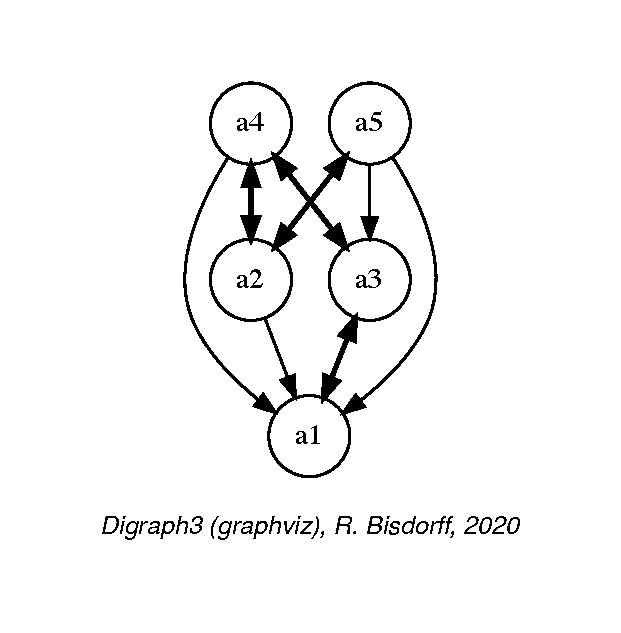
\includegraphics[width=7cm]{Figures/1-1-tutorialDigraph.pdf}
\caption[The tutorial crisp digraph]{The tutorial crisp digraph. The \texttt{exportGraphViz()} method is depending on drawing tools from \texttt{https://graphviz.org}. On Linux Ubuntu or Debian you may try '\texttt{sudo apt-get install graphviz}’ to install them. For Mac OSX There are ready $dmg$ installers available}
\label{fig:1.1}       % Give a unique label
\end{figure}

Further methods are provided for inspecting this random \texttt{Digraph} object \texttt{dg}, like the following \texttt{showStatistics()}\index{showStatistics@\texttt{showStatistics()}} method.
\begin{lstlisting}[caption={Inspecting a \texttt{Digraph} object},label=list:1.5]
>>> dg.showStatistics()
 *----- general statistics -------------*
 for digraph              : <tutorialDigraph.py>
 order                    : 5 nodes
 size                     : 12 arcs
 undetermined           : 0 arcs
 determinateness (%)      : 100.0
 arc density              : 0.60
 double arc density       : 0.40
 single arc density       : 0.40
 absence density          : 0.20
 strict single arc density: 0.40
 strict absence density   : 0.20
 nbr. of components         : 1
 nbr. of strong components  : 1
 transitivity degree (%)  : 60.0
                          : [0, 1, 2, 3, 4, 5]
 outdegrees distribution  : [0, 1, 1, 3, 0, 0]
 indegrees distribution   : [0, 1, 2, 1, 1, 0]
 mean outdegree           : 2.40
 mean indegree            : 2.40
                          : [0, 1, 2, 3, 4, 5, 6, 7, 8, 9, 10]
 symmetric degrees dist.  : [0, 0, 0, 0, 1, 4, 0, 0, 0, 0, 0]
 mean symmetric degree    : 4.80
 outdegrees concentration index   : 0.1667
 indegrees concentration index    : 0.2333
 symdegrees concentration index   : 0.0333
                                  : [0, 1, 2, 3, 4, 'inf']
 neighbourhood depths distribution: [0, 1, 4, 0, 0, 0]
 mean neighbourhood depth         : 1.80
 digraph diameter                 : 2
 agglomeration distribution       :
 a1 : 58.33
 a2 : 33.33
 a3 : 33.33
 a4 : 50.00
 a5 : 50.00
 agglomeration coefficient        : 45.00
\end{lstlisting}

The preceding \texttt{show...()} methods usually rely upon corresponding compute methods, like: \texttt{computeSize()}\index{computeSize@\texttt{computeSize()}}, \texttt{computeDeterminateness()}\index{computeDeterminateness@\texttt{computeDeterminateness()}},\\ or \texttt{computeTransitivityDegree()}\index{computeTransitivityDegree@\texttt{computeTransitivityDegree()}}.
\begin{lstlisting}[caption={Various \texttt{compute...()} methods.},label=list:1.6]
>>> dg.computeSize()
 12
>>> dg.computeDeterminateness(InPercents=True)
 Decimal('100.00')
>>> dg.computeTransitivityDegree(InPercents=True)
 Decimal('60.00')
\end{lstlisting}

Mind that \texttt{show...()} methods output their results in the \emph{Python} console. We provide also some \texttt{showHTML...()} methods which output their results in a system browser’s tab or window.
\begin{lstlisting}
>>> dg.showHTMLRelationMap(relationName='r(x,y)',\
...                        rankingRule=None)
\end{lstlisting}
\begin{figure}[ht]
\sidecaption[t]
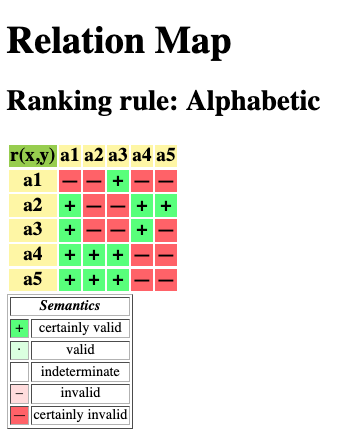
\includegraphics[width=5cm]{Figures/1-2-relationMap1.png}
\caption[Browsing the relation map of the tutorial digraph]{Browsing the relation map of the tutorial digraph. $+$ indicates a certainly valid and $-$ indicates a certainly  invalid relation, Here we find confirmed again that our random digraph instance \texttt{dg}, is indeed a crisp, i.e. $100\%$ determined irreflexive digraph instance}
\label{fig:1.2}       % Give a unique label
\end{figure}

% \section{Special digraph instances}
% \label{sec:1.5}

Some special types of digraph instances, like the \texttt{CirculantDigraph}\index{CirculantDigraph@\texttt{CirculantDigraph} class} or the \texttt{GridDigraph}\index{GridDigraph@\texttt{GridDigraph} class} classes, are readily available (see Fig.~\vref{fig:1.3}).
 \begin{figure}[ht]
%\sidecaption[t]
  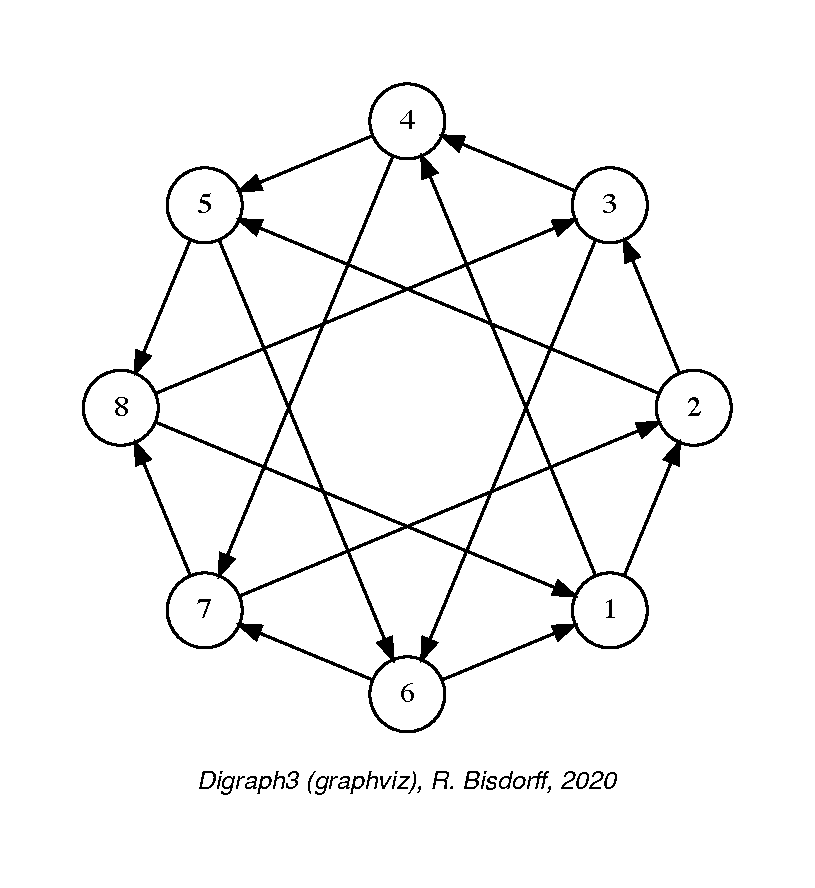
\includegraphics[height=6cm]{Figures/1-3-c8.pdf} \hfill
  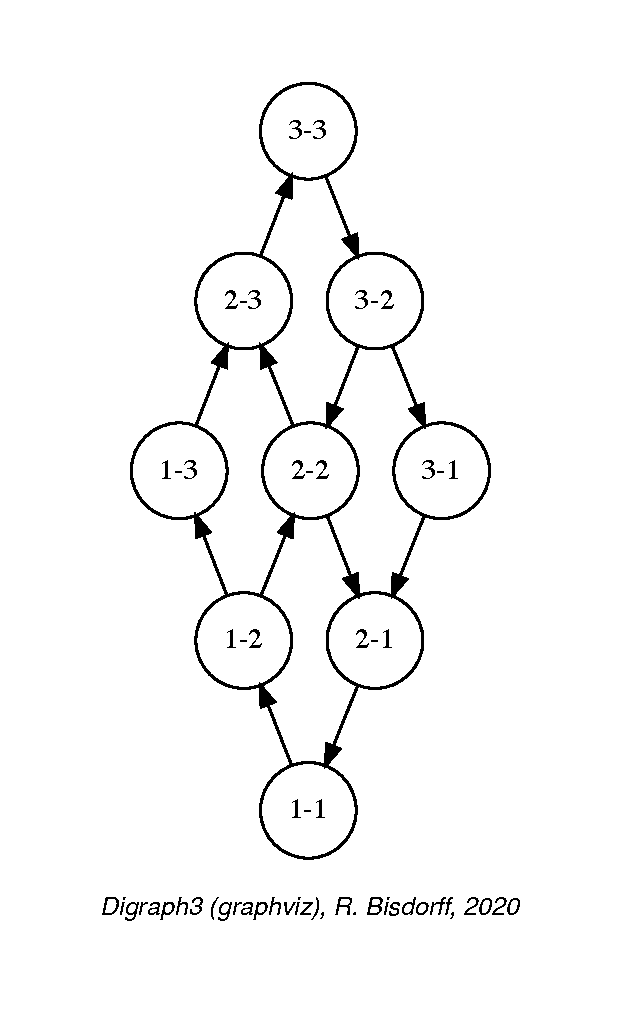
\includegraphics[height=6cm]{Figures/1-3-grid3.pdf} \hfill
  \caption{The circulant [1,3] digraph and the 3x3 grid digraph}
\label{fig:1.3}       % Give a unique label
\end{figure}
\begin{lstlisting}[caption={Circulant digraphs and $n \times m$ grid digraphs},label=list:1.7]
>>> from digraphs import CirculantDigraph,GridDigraph
>>> c8 = CirculantDigraph(order=8,circulants=[1,3])
>>> c8.exportGraphViz('c8')
  *---- exporting a dot file for GraphViz tools ----*
   Exporting to c8.dot
   circo -Tpng c8.dot -o c8.png
>>> grid3 = GridDigraph(n=3,m=3,\
...                    hasMedianSplitOrientation=True)
>>> grid.exportGraphViz('grid3')
  *---- exporting a dot file for GraphViz tools ----*
   Exporting to grid3.dot
   dot -Grankdir=BT -Tpng grid3.dot -o grid3.png
 \end{lstlisting}

%\vspace{1cm}
\vspace{\baselineskip}
The next Chapter~\ref{sec:2} will introduce the fondamental \emph{bipolar-valued digraph} model which is \emph{root object type} to all the digraph models implemented in the \Digraph modules \citep{BIS-2021b}.    

%%%%%%% The chapter bibliography
% % \normallatexbib
%\phantomsection
%\addcontentsline{toc}{section}{Chapter Bibliography}
%\input{02-mainMatters/01-chapterIntroDigraph3.bbl}
\bibliographystyle{spbasic}
\bibliography{03-backMatters/reference}

\bibliographystyle{spbasic}
\bibliography{03-backMatters/reference}

\bibliographystyle{spbasic}
\bibliography{03-backMatters/reference}
